
\begin{description}
    \item[\textsc{Source}]  Paper delivered at the Human Behavior and Evolution Society Annual Meeting, 2016, in a session "Macroevolutionary Approaches to Cultural and Technological Evolution."  
    \footnote{Archived as \url{https://figshare.com/articles/madsen2016-hbes-computational-interaction-patterns-slides_pdf/3468650}.}
    \end{description}
    
    %%%%%%%%%%%%%%%%%%%%%%%%%%%%%%%%%%%%%%%%%%%%%%%%%%%%%%%%%%%%%%%%%%%%%%%%%%%%%%%%%%%%%%%%%
    
    \section{Introduction}\label{metapop:sec:introduction}
    
    One of the most important tasks of an evolutionary archaeology is documenting evolutionary history itself.  This means more than creating chronology and documenting the history of material culture change, although those are essential tasks.  Without the ``chronicle'' \citep{OHara1988} of empirical facts, we cannot construct the testable narratives that represent the evolution of culture.  But evolutionary history requires more than documenting chronology and change in artifact types and assemblages; it requires inference of \emph{heritable continuity} from the ``mere facts'' of \emph{historical continuity} in artifact classes \citep{o2000applying}.  Doing so requires separating similarity which represents \emph{homology}---similarity due to descent---from convergence due to natural selection but without common descent \citep{Dunnell1978,kroeber1931historical}.  
    
    Dunnell \citeyearpar{Dunnell1978,Dunnell1980,dunnell1989aspects} argued that despite lacking a real theoretical basis for the endeavor, early culture historians had developed intuitive methods for tracing heritable continuity \citep{o2000applying,lyman1997rise}.  In modern terms, the core methods of culture history such as Krieger's \citeyearpar{Krieger1944} ``test of historical significance'' and seriation \citep{Dunnell1970,Ford1935,Ford1936,Ford1949} allow the tracing not just of chronology, but provides evidence of heritable continuity and thus the history of past cultural transmission \citep{lyman2008cultural}.
    
    At the largest spatiotemporal scales, phylogenetic methods are replacing the traditional tools of culture history for framing hypotheses about the chronicle of cultural change at the largest scales  \citep{borgerhoff2006cultural,Lyman1997a,Lyman2006a,o1999seriation,o2000time,o2001cladistics,o2003cladistics,o2003resolving,OBrian2000,prentiss2019cultural,PRENTISS201564,Temkin2007}.  The ``resolution'' of methods like phylogenetic analysis depends upon the nature of the classifications employed, and the fact that analyses typical employ only presence/absence data rather than detailed class frequencies.  Especially because class presence/absence is the typical criterion for splitting on trees, most uses of phylogenetic methods in archaeology are ``macroevolutionary'' \citep{prentiss2019cultural}.  
    
    When we wish to operate at smaller scales and over shorter amounts of time, we need methods that employ not just presence/absence information about classes and types, but all of the frequency and spatial information at our disposal.\footnote{This is not to say that cladistic methods are not applicable to mesoscale analysis, but they may require custom classifications with finer levels of ``splitting'' of attributes.}  This is especially true in the archaeology of the late Holocene, when we wish to resolve events that might represent change over decades rather than centuries, and within smaller study areas.  This level of detail has long been part of archaeology, with regional studies and syntheses like Ford's work in the Vir\'u Valley of Peru \citep{Ford1949} and Phillips, Ford, and Griffin's \citeyearpar{PFG1951} study of the Lower Mississippi River Valley.  More recently under the ``New Archaeology,'' work at this scale was often included under the general umbrella of ``regional analysis'' \citep{johnson1977aspects}.  When focused on tracing the history of cultural transmission, at the spatial and temporal scales mentioned, I call this kind of analysis ``mesoscopic,'' since it lives in an intermediate zone between the ``microevolutionary'' study of single assemblages or localities, and the ``macroevolutionary'' focus of much larger scale and comparative work.  
    
    The core methods of culture history, and especially seriation, were designed precisely to answer questions about chronology and cultural transmission at mesoscopic and macroevolutionary scales, but in intuitive ways with common-sensical explanatory concepts such as ``trade'' and ``migration'' \citep{o2000applying,lyman1997rise,lyman2008cultural}.  Because the end products were atheoretical and interpretive, there was little reason to develop a more detailed quantitative understanding of what could be done with methods like seriation, and when radiometric dating methods arrived on the scene, it was easy to frame seriation as nothing more than a ``relative dating method'' instead of a generalized method for tracing homology, \emph{which just happened} to deliver temporal information as a side effect.  
    
    This paper builds upon previous work by myself and Carl Lipo reformulating seriation in a rigorous way to focus on the tracing of homology and construction of evolutionary chronicles  \citep{Lipo1997,Lipo2001,Lipo2015,Madsen2008} and Chapter \ref{chap:multipleseriation-paper}. In this work, I focus on the question of how seriation graphs, output from our iterative deterministic seriation algorithm (IDSS), can function as observable data in fitting scenarios for the history of cultural transmission at regional scales.  The goal is to build a computational and statistical approach to describe \begin{dissparalist}
    \item the structure of cultural relatedness within a region  
    \item our hypotheses about the cultural transmission history 
    \end{dissparalist} in quantitative ways that allow us to use standard machine learning and statistical tools to perform model selection and assess goodness-of-fit.  
    
    This paper introduces ``interval temporal networks'' as the natural data structure for representing our hypotheses about the history of cultural transmission.  Simulation of cultural transmission on interval temporal networks provides samples of the distribution of cultural traits we would expect to see for a given hypothesis.  Seriation graphs can be constructed both for the simulation output of each hypothesis, and for our empirical data from archaeological assemblages.  We then extract summary graph metrics for seriation graphs, allowing us to describe their structure in quantitative terms suitable for a machine learning classifier to be used to assess \begin{dissparalist}
    \item the identifiability of different cultural transmission hypotheses given seriation graphs (i.e., their equifinality between hypotheses)
    \item the transmission hypothesis for which our empirical seriation graphs have the closest match
    \end{dissparalist}.
    
    The results reported here are preliminary but encouraging.  Using seriations as the observable variable alone, it is possible to differentiate between regional transmission histories where communities are largely balanced in their interaction and interact with all their peers, from histories that show very localized, ``nearest neighbor'' interaction, from histories involving the coalescence of different lineages, or their splitting to form two or more groups which no longer interact.  I examine these scenarios with respect to our previous seriation results for Mississippian ceramic assemblages in the Central and Lower Mississippi River Valley.   
    
    \section{Documenting the Regional History of Cultural Transmission With Seriation Graphs}\label{metapop:sec:seriation-graphs}
    
    The culture-historical seriation method employs an ordering criterion, either continuity of class presence/absence, or unimodality of class frequencies, to provide a relative chronological order.  It does so under an assumption that the ``correct'' order will be the one that introduces no discontinuities in any of the classes used in the ordering \citep{Ford1949,PFG1951,Rouse1939}.  This means that in occurrence seriation, the correct order will not contain gaps where classes exist in a region, go away, and then come back.  Instead, all classes will display continuous existence throughout their respective lifetimes.  For frequency seriation, the correct order will not display situations where some classes have discontinuous ``jumps'' in frequency value inconsistent with their local trend.  These assumptions are what one would expect if seriation is providing a relative history of how different cultural traits, expressed as archaeological classes or types, were learned and inherited within a population or populations in a region.
    
    Several things can disturb our ability to cleanly order a set of samples into a single linear, chronological relationship.  \citet{Dunnell1970} describes these, and the criteria traditionally used to minimize them and produce usable seriations.  First, we expect all of the assemblages to represent comparable durations of time, otherwise some will be time averaged over a longer history of transmission and cultural change than others, and not be orderable with the rest.  Second, in a traditional seriation we minimize the amount of spatial variation involved, since cultural traits flow across space as well as time.  If we want seriations to only depict the chronological relationships, we must minimize the amount of spatial variation we include \citep{PFG1951,Rouse1967}.
    
    If our goal, on the other hand, is not to extract just chronology, but understand the spatio-temporal history of how cultural traits spread within a region, then we need to do several things.  First, we need to stop trying to force the seriation to yield a single linear order.  Instead, if there are multiple valid ways that the frequencies of the classes can be arranged, we should express these as individual possible ``solutions''.  In our 1997 paper with Tim Hunt and Robert Dunnell \citeyearpar{Lipo1997}, we proposed breaking seriation solutions into multiple subsets, with the unimodality (or occurrence) criterion applied strictly within each subset.  This allows deterministic solutions (\emph{sensu} \citealt{Dunnell1970,Dunnell1981}) which are temporal within each subset, while the differences between subsets reflects spatial variation in the history of cultural traits.  Some classes may increase in frequency spreading to the north, for example, at the same time that the same classes are declining in frequency in a southern direction.  Attempting to incorporate both patterns in the same linear ordering will result in no solution (or, in the case of multivariate statistical methods, a low confidence solution with much ``noise'' whose utility is entirely unclear).  
    
    \citet{Lipo2001} took another step towards formalizing seriation in his dissertation by investigating methods for assessing the quality of a proposed solution.  He employed a bootstrap resampling approach to estimate the likely standard error around frequency estimates given the overall sample size we possess for a site or assemblage.  This allows us to assign a confidence interval to each  ``bar'' in a frequency seriation.  Confidence intervals can then be used to \begin{dissparalist}
    \item perform pairwise comparisons between assemblages to assess the significance of an ordering 
    \item understand quantitatively which assemblages are ``contemporaneous'' in the sense that the data at hand cannot distinguish between them
    \end{dissparalist}.  
    
    \begin{figure}[ht]
    \centering
    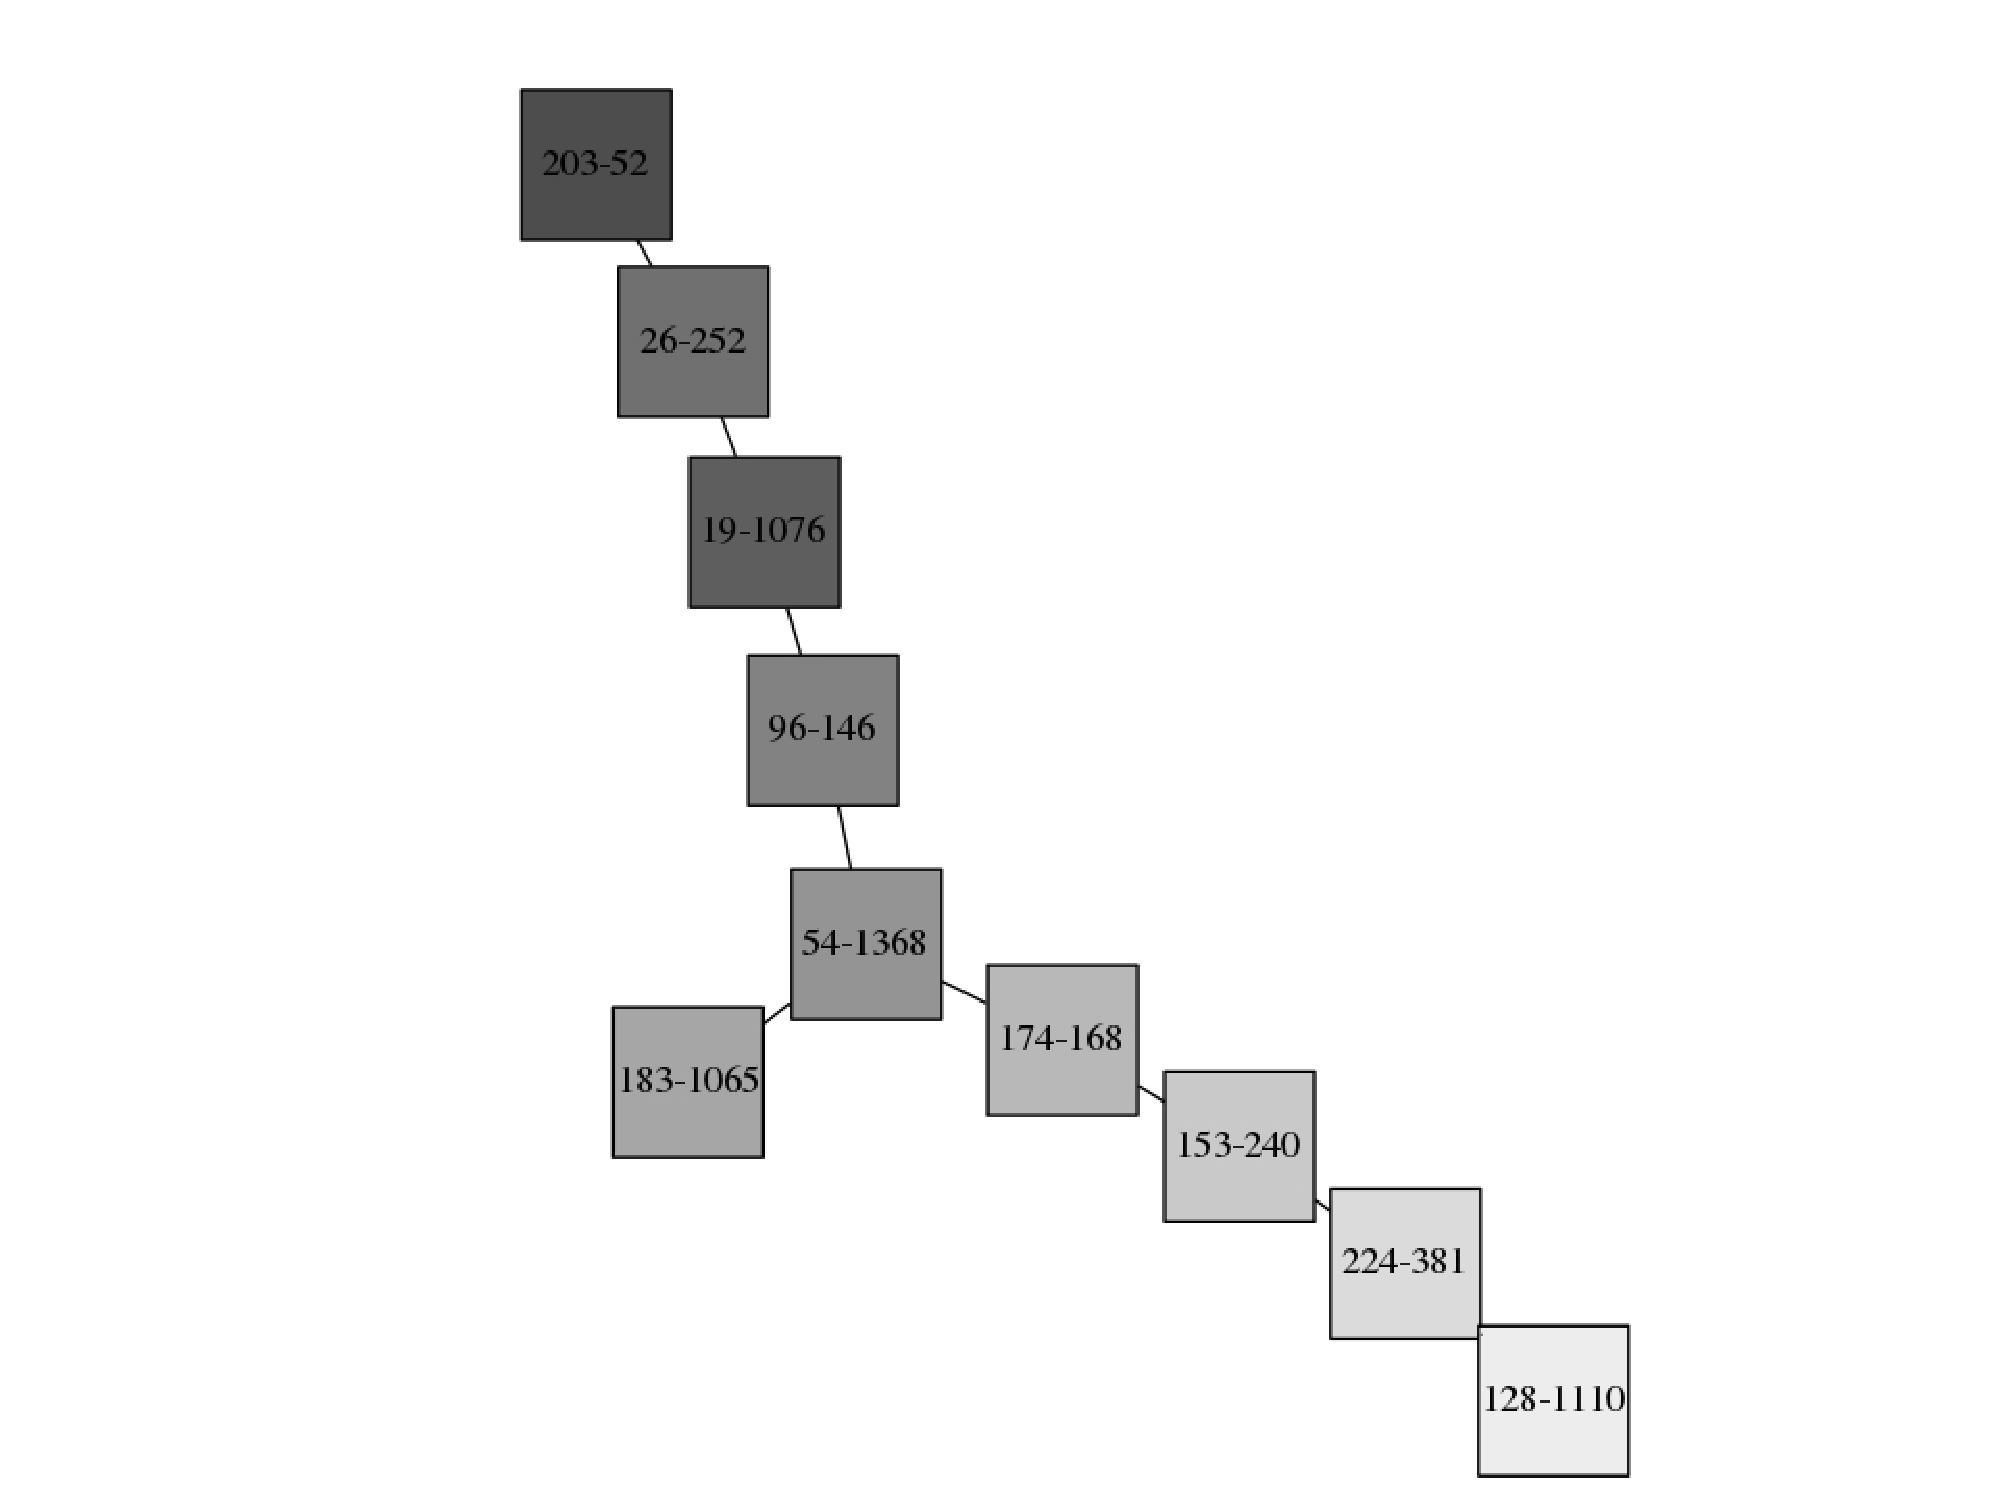
\includegraphics[scale=0.40]{graphics/multipleseriation/example-graph-branching-seriation.pdf}
    \caption{Example of a seriation graph, which represents two separate seriation solutions, with one assemblage (54-1368) represented in both subsets.  When overlaid, the separate solutions form a graph rather than a single linear ordering.  Shading of assemblages reflects temporal information, with light as early and late as dark.}
    \label{metapop:fig:seriation-graph-example}
    \end{figure}
    
    The ability to test significance of ordering decisions and detect contemporaneity provided the tools to perform an automated breakdown of seriation solutions into multiple solutions, as we proposed in our early work to capture both spatial and temporal information.  In our 2015 paper describing the IDSS algorithm \citep{Lipo2015}, we took the additional step of representing the relationship between each subset in a seriation with multiple possible solutions.  Whenever an assemblage is present in two or more subset solutions, we link the linear subsets together into a graph, at the assemblage which appears in both.  Figure \ref{metapop:fig:seriation-graph-example} shows an example of such a graph, which merges two possible solutions from a simulation of cultural transmission with spatial structure.  
    
    The ability to use seriations as observable data, to which we directly fit hypotheses about the history of cultural transmission, requires that seriations be large enough, and encompass enough spatial and temporal variation, that there is meaningful \emph{structure} to the resulting graphs.  If every seriation we perform has only a few assemblages and comes out as a linear or near-linear order, seriations will \emph{underdetermine} our hypotheses.  Thus, we need to be able to find valid solutions with dozens of assemblages, at least, if not more.  It is well known that the basic brute-force seriation problem faces a combinatorial explosion of possibilities, and as described in Chapter \ref{chap:seriationcombinatorics-paper} breaking the solution into subsets or general graphs only makes the number of possible solutions larger.  Lipo and I revisited earlier work by \citep{Kadane1971} and added distance minimization as a criterion to our seriation algorithms, allowing much larger sets of assemblages to be ordered than with the frequency criterion, but yielding identical results in nearly all cases.  That work is reported in Chapter \ref{chap:multipleseriation-paper}.  
    
    These methodological revisions to seriation yield a method whose output---seriation graphs---are comparable to phylogenetic trees in tracing the structure of homology, but doing so with all of the frequency information at our disposal.  Seriation graphs thus complement phylogenetic trees at the mesoscopic level of analysis.  Each seriation graph documents the ``evolutionary chronicle'' of how cultural traits were transmitted through a region by teaching and learning of the young, migration, marriage and kinship structure, and trade.  The seriation graph is an ``observable variable'' which we can analyze, cluster, and potentially fit to models which describe the history of cultural transmission at regional scales.
    
    
    
    \section{Representing Hypotheses About Regional Transmission History With Temporal Networks}\label{metapop:sec:temporal-networks}
    
    In order to assess that fit, we need to express our hypotheses about regional history in a quantitative, structured way.  
    We must frame hypotheses about the regional history of cultural transmission which are appropriate given the kind of aggregated, coarse-grained data we are able to possess.  For purposes of this study, I focus on one particular kind of empirical case:  the archaeological record of nucleated, sedentary communities.  In such cases, we tend to have data on artifact class frequencies from ``sites'' or partitions of sites, sometimes over subsets of the complete interval of occupation, but at the very least, covering the entire occupation duration.  At worst, our assemblages thus represent an aggregation over some local population, over some period of time.  The frequencies of cultural traits we have to work with are thus coarse-grained at the population level, and time averaged.  
    
    This means that we have to model the history of how cultural traits were transmitted at the same level of detail or higher.  We can model this in the form of a graph \citep{diestel2010graph,Harary1969}.  Graph representations have been used for decades in archaeology \citeeg{hunt1988graph,irwin1977network,Mills2010,mills2017social,terrell1977human}. We can represent the presence of transmission---via any mechanism, whether flows of people by migration or intermarriage, trade, observation and imitation of one's neighbors---simply as a link between two vertices.  If we can somehow measure the relative intensity, averaged over time, of the flow or adoption of cultural traits between two communities, we can represent that as a numerical ``weight'' on the edges of the graph.  So far this is standard static graph theory as employed in the growing field of ``social network analysis.''  
    
    But to represent \emph{history} we need to represent time in the graph, which most applications of social network analysis both inside and outside archaeology have been slow to do.  We can incorporate time by creating a \emph{time-varying} or \emph{temporal} network model \citep{Holme2012}.  Temporal network models add a time dimension to graph models by recognizing that edges may change their weight, or even their presence and absence, and that vertices may go away or arise at various points in time.  Temporal networks can be represented in two ways, depending upon the nature of the ``contact''' they represent.  If an edge represents an instantaneous event (from the perspective of the overall model), we refer to the resulting model as a ``contact network''.  If we model edges as having non-trivial durations, the resulting model is an ``interval network.''  Contact networks are a useful framework for studying individual-level behavior, constructing realistic epidemiological models, or gene expression and protein regulatory networks in cell biology, for example \citep{holme2012temporal}.  For our purposes in archaeology, interval temporal networks will be most useful, since we need to represent the duration over which each set of class frequency observations spans.  
    
    \begin{figure}[ht]
    \centering
    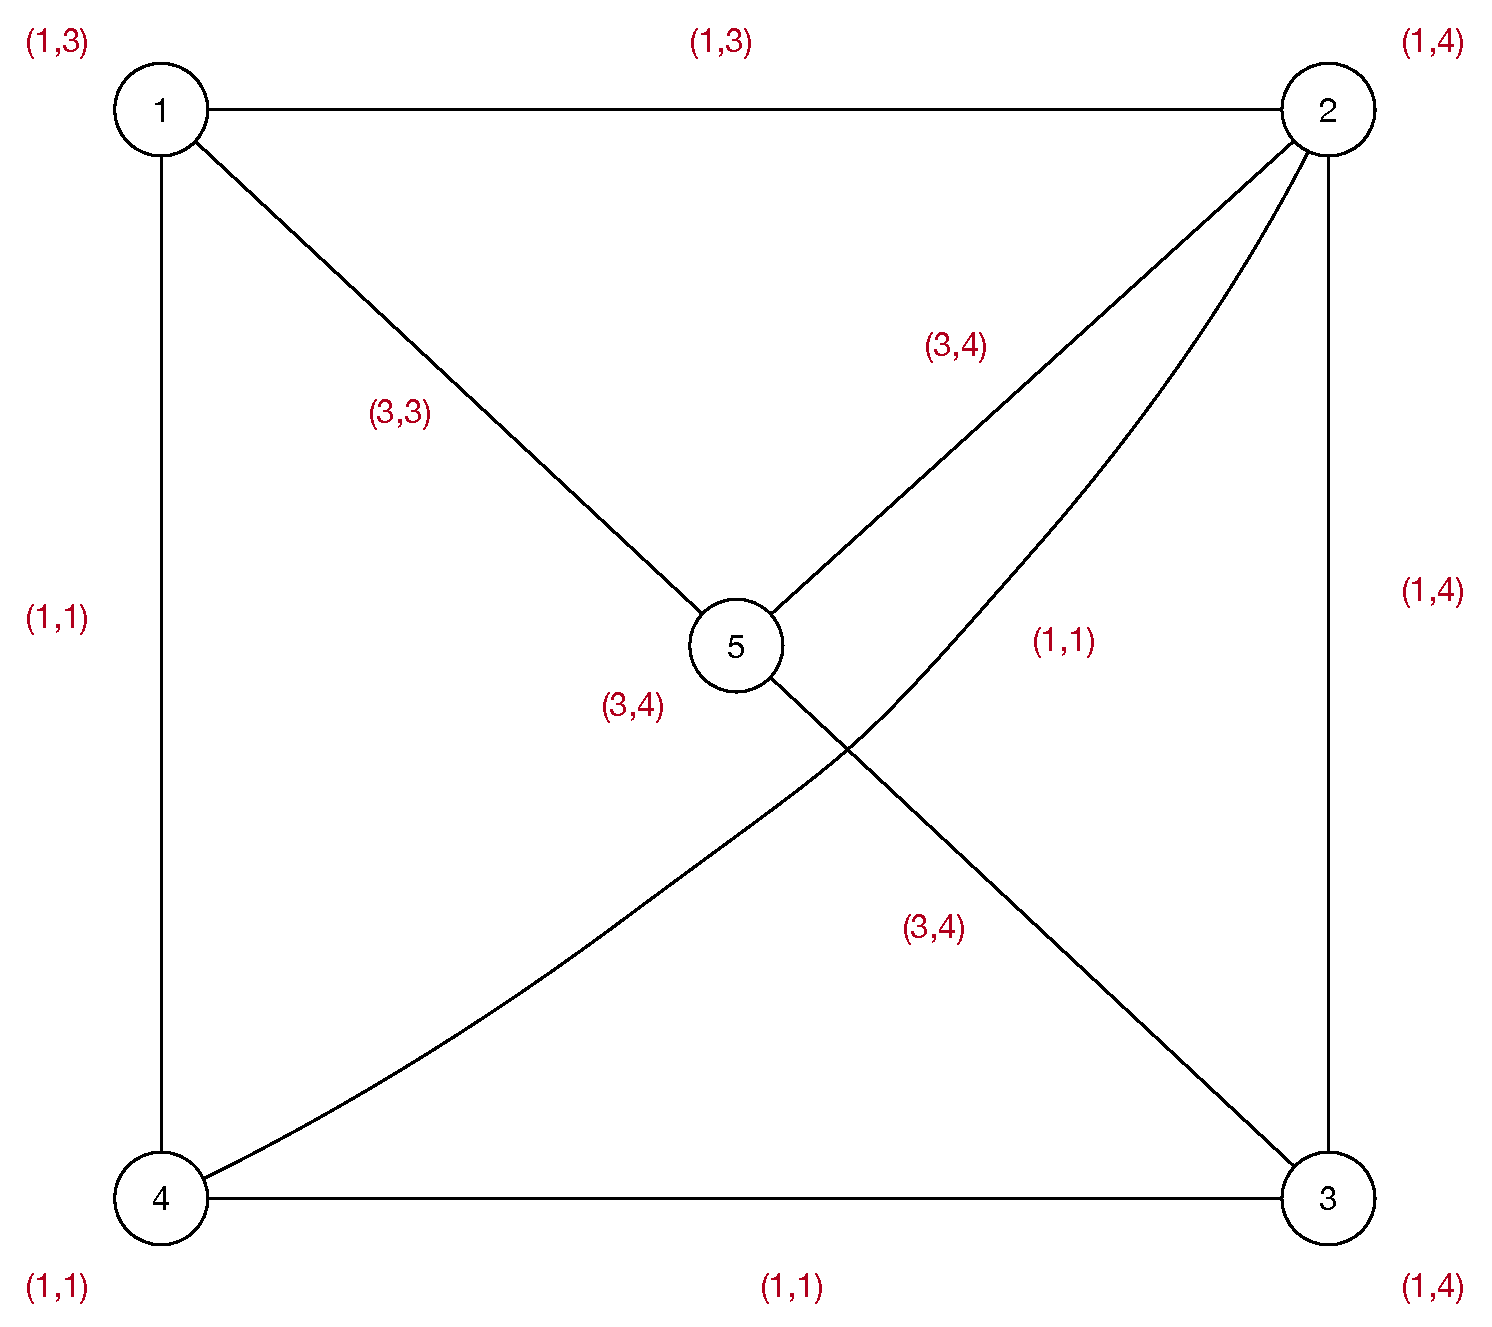
\includegraphics[scale=0.50]{graphics/multipleseriation/interval-temporal-network-single-view.pdf}
    \caption{Example of an interval temporal network, viewed as a single graph object.  In addition to the familiar vertices and edges of a non-temporal graph, each vertex and edge is annotated with the intervals of time over which that object existed.  Time in this simple example is arbitrary, and simply represents times at which change events occur.}
    \label{metapop:fig:itn-single-example}
    \end{figure}
    
    An interval temporal network (ITN) is a graph \(G\) with vertex set \(V\), where each vertex \(v\) specifies a tuple \((t, \delta t)\), which denotes the time index and duration for which each vertex exists, and an edge set \(E\), where each edge carries a tuple \(w, t, \delta t)\), giving the edge weight and the time index and duration over which that edge exists with that weight value.  Visualizing this graph is very difficult all at once, since most of the information about the structure of the graph at any point in time is carries in numbers associated with each vertex and edge (Figure \ref{metapop:fig:itn-single-example}).  
    
    Instead, it is convenient both visually and when operating on an ITN computationally to decompose the single model into a sequence of separate graphs.  Each graph \(G_t\) in the sequence represents one
    or more change events within the network between times \(t_i\) and
    \(t_j\) where \(i\) and \(j\) represent the union of ``change'' events in the temporal attributes from the vertex and edge sets.  In other words, every addition or loss of an edge or vertex triggers a new \(G_t\) in the sequence, and each subgraph in the temporal sequence describes the state of the ITN in terms of vertices and edges over some duration of time where we can observe no change (given the resolution of the data we possess).  We must assume that there is an unknown amount of fine-grained change occurring over the interval represented by each subgraph \(G_t\) but that variation is not available to us; in this way, the interval temporal network representation ``naturally'' allows us to incorporate the time averaging and coarse-graining of our observed data as part of our observational model.  Figure \ref{metapop:fig:itn-sliced-example} displays the same interval temporal network as Figure \ref{metapop:fig:itn-single-example}, but decomposed into a series of ``slices'' through time at change points, as vertices go away and a new one arises, with changes in the pattern of connectivity.
    
    \begin{figure}[ht]
    \centering
    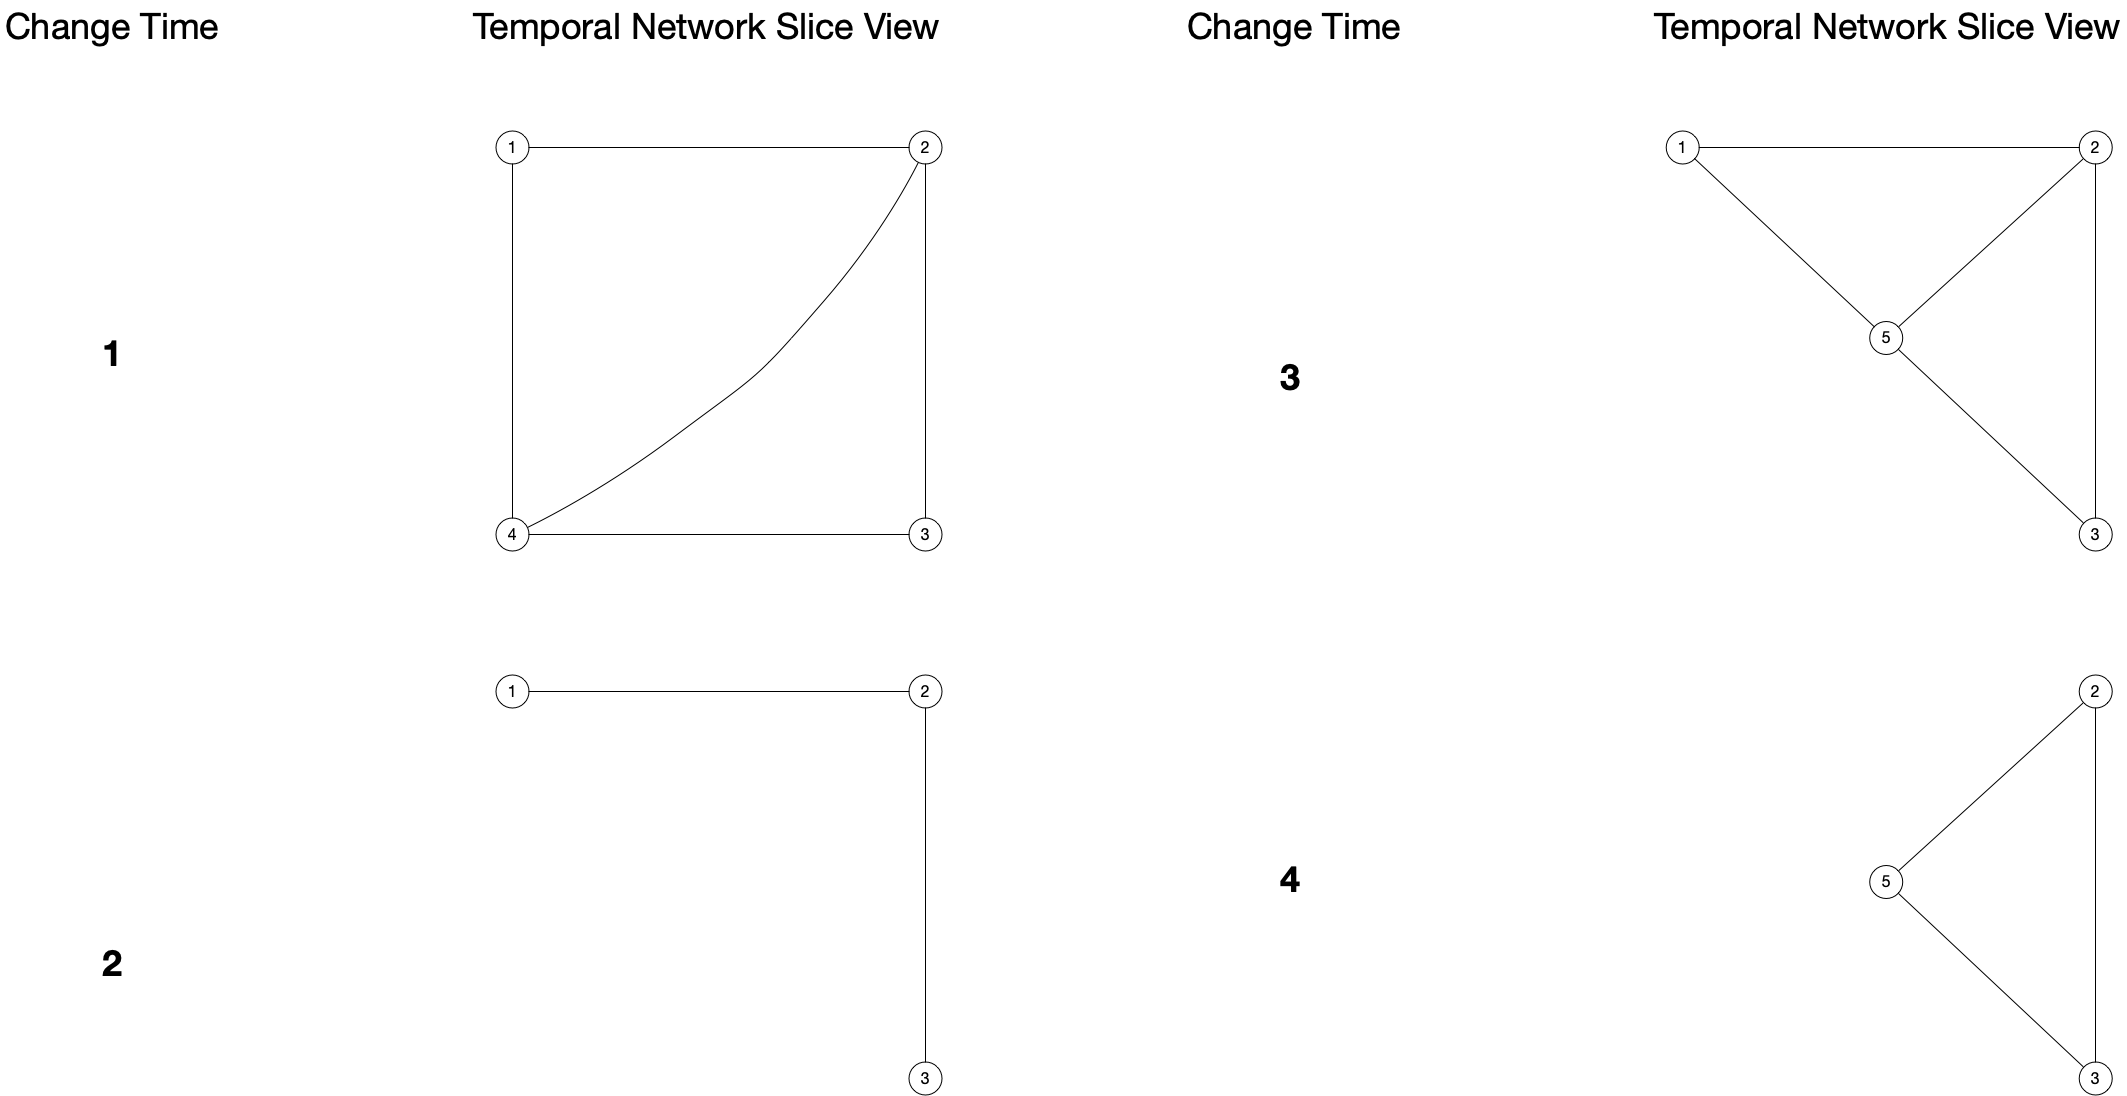
\includegraphics[scale=0.20]{graphics/multipleseriation/interval-temporal-network-sliced-view.png}
    \caption{Example of an interval temporal network, viewed as a series of ``slices'' at time indices that represent structural changes.  Time in this simple example is arbitrary, and simply represents times at which change events occur.}
    \label{metapop:fig:itn-sliced-example}
    \end{figure}
    
    The interval temporal network is thus a tool for representing networks or interaction patterns not just at a point in time (as in most uses of graph theory for social network analysis) but as those relationships evolve and change.  This gives us a way to represent models or hypotheses about how the structure of cultural transmission and regional interaction may have changed, in particular regions or areas.  
    
    Such scenarios are necessarily coarse-grained, like our data, and would represent the the flow of cultural traits, whether through the flow of people, material objects, as pure information, by edges in the graph.  Vertices represent communities or subpopulations in particular places.  The samples of artifacts we obtain archaeologically provide us temporally aggregated  samples of cultural variation from those communities.  Because that information is time averaged, we represent that duration as the start and end times for the vertex in the ITN.  
    
    In our hypotheses about evolutionary history in a region, we can represent different scenarios about how information flows by the way we choose to represent edges in our models.  If communities were in contact with most of their neighbors and there is no strong hierarchical pattern, as we might expect in early agricultural communities of the Late Woodland for example, then we could model this with even edge weights.  If communities largely interacted with those around themselves, with a smaller number of long-distance links (perhaps for exogamous marriages), we might expect a more lattice-like pattern of ``nearest neighbor'' edges.  The hierarchical structures posited for the ``complex'' Mississippian communities of eastern North America might imply edge patterns structured such that certain edges had stronger weight than others.  These patterns then need to be modeled in the temporal dimension:  we can explicitly model the process of small agricultural communities aggregating to form larger and more hierarchical units, and examine the consequences for cultural transmission and the pattern of cultural variation it might leave behind.  We can model the process of the development of separate, divergent ``traditions'' in a region, or the process of several independent ``lineages'' coalescing to form a larger group.   
    
    In the representation developed here, each interval temporal network \(G\) as a whole (not its subgraphs) represents a single possible ``history'' of the presence, absence, and intensity of the sharing of cultural traits between communities over time, as well as the timing and duration of the archaeological assemblages representing those communities.  There are many possible histories, and our goal is to find sets of histories which most closely match the empirical data we have concerning cultural trait frequencies in these assemblages.  The notion of a ``set of histories'' is important, because at a detailed level even if we have good knowledge of the vertex set (e.g., all of the Mississippian town sites in the central Mississippi River valley) and their durations of occupation, there may be many possible ITN models which correspond to the similarities and sequences of changes in class frequencies that we observe.  Additionally, the vertex set we operate with always represents a sample of the full archaeological record, since our knowledge of that record is incomplete, parts of the record have been fully destroyed by contemporary development, or are otherwise unavailable for study.  Thus, we are always examining \emph{equivalence classes} of transmission scenarios.  As individual models, the members of an equivalence class are equifinal with each other given the data we possess, and the data we posses underdetermines any distinctions between individual models.  
    The question thus arises:  what kind of transmission scenarios can we distinguish using the kind of coarse-grained, time averaged data on artifact class frequencies we typically possess?  In this paper I study that issue from a theoretical perspective in order to build a statistical and computational approach to identifying the class of transmission scenarios which fit the data from a case study using ceramic assemblages from the Lower Mississippi River Valley (Section \ref{metapop:sec:results-lmv}).  
    
    \subsection{Transmission Scenarios Studied}\label{metapop:sec:transmission-scenarios}
    
    In this study, I employ very coarse-grained transmission scenarios, of the kind just described.  The scenarios considered here are simple ones:
    
    \begin{itemize}
        \item Complete networks:  all communities exchange information and individuals with each other;
        \item Nearest neighbor networks:  Interaction is strongly or weakly biased toward nearest neighbors, with small numbers of longer distance links;
        \item Lineage splitting:  a single complete network loses enough links that non-communicating subsets are formed which evolve on their own;
    \end{itemize}
    
    Nearest neighor networks were examined in two variants, to see if the actual spatial arrangement can be distinguished.  One model was long and thin (``rectangular nearest neighbor'') to mimic communities interacting only with their neighbors up and down a river, for example.  A second model was square (``square nearest neighbor'') to provide most communities with interacting neighbors in all directions.  With an example of a complete network where every community interacted with all others, and a lineage-splitting example where an initial large population splits into two non-interacting lineages, these form the scenarios considered in the present study.
    
    These four scenarios are very basic, and obviously do not encompass the full range of regional histories we might wish to examine for a region as richly complex as the late prehistoric Mississippi River valley.  For example, the interaction pattern between mound center and residential sites, and the relative size of mounds underlies a lot of the discussion around social complexity in the Mississippian of the American southeast \citep{blitz2010new,cobb2003mississippian,Lipo2001a,Lipo2001}.  An ideal outcome of the line of inquiry pursued in this study would be that large enough sets of assemblages, analyzed into seriation graphs \citep{Lipo2015}, would be comparable to transmission scenarios which represent hierarchical patterns of information flow.   This study focuses on the coarse-grained scenarios described here, principally because  development of the conceptual and computational methods needed.  Future work will need to focus on more precise ways of expressing our archaeological hypotheses in the form of interval temporal networks, and understanding the tradeoffs of different ways of representing something like hierarchy.
    
    For each of the general scenarios described in this section, I constructed interval temporal networks that exhibited that structure.  An illustration is shown in Figure \ref{metapop:fig:itn-example} provides an example of a ``decomposed'' representation of a ``lineage splitting'' scenario, where a regional population, with two subpopulations that interact to a limited extent earlier in prehistory, become largely separate in their cultural repertoires over time through loss of direct cultural transmission.  
    
    \begin{figure}[ht]
    \centering
    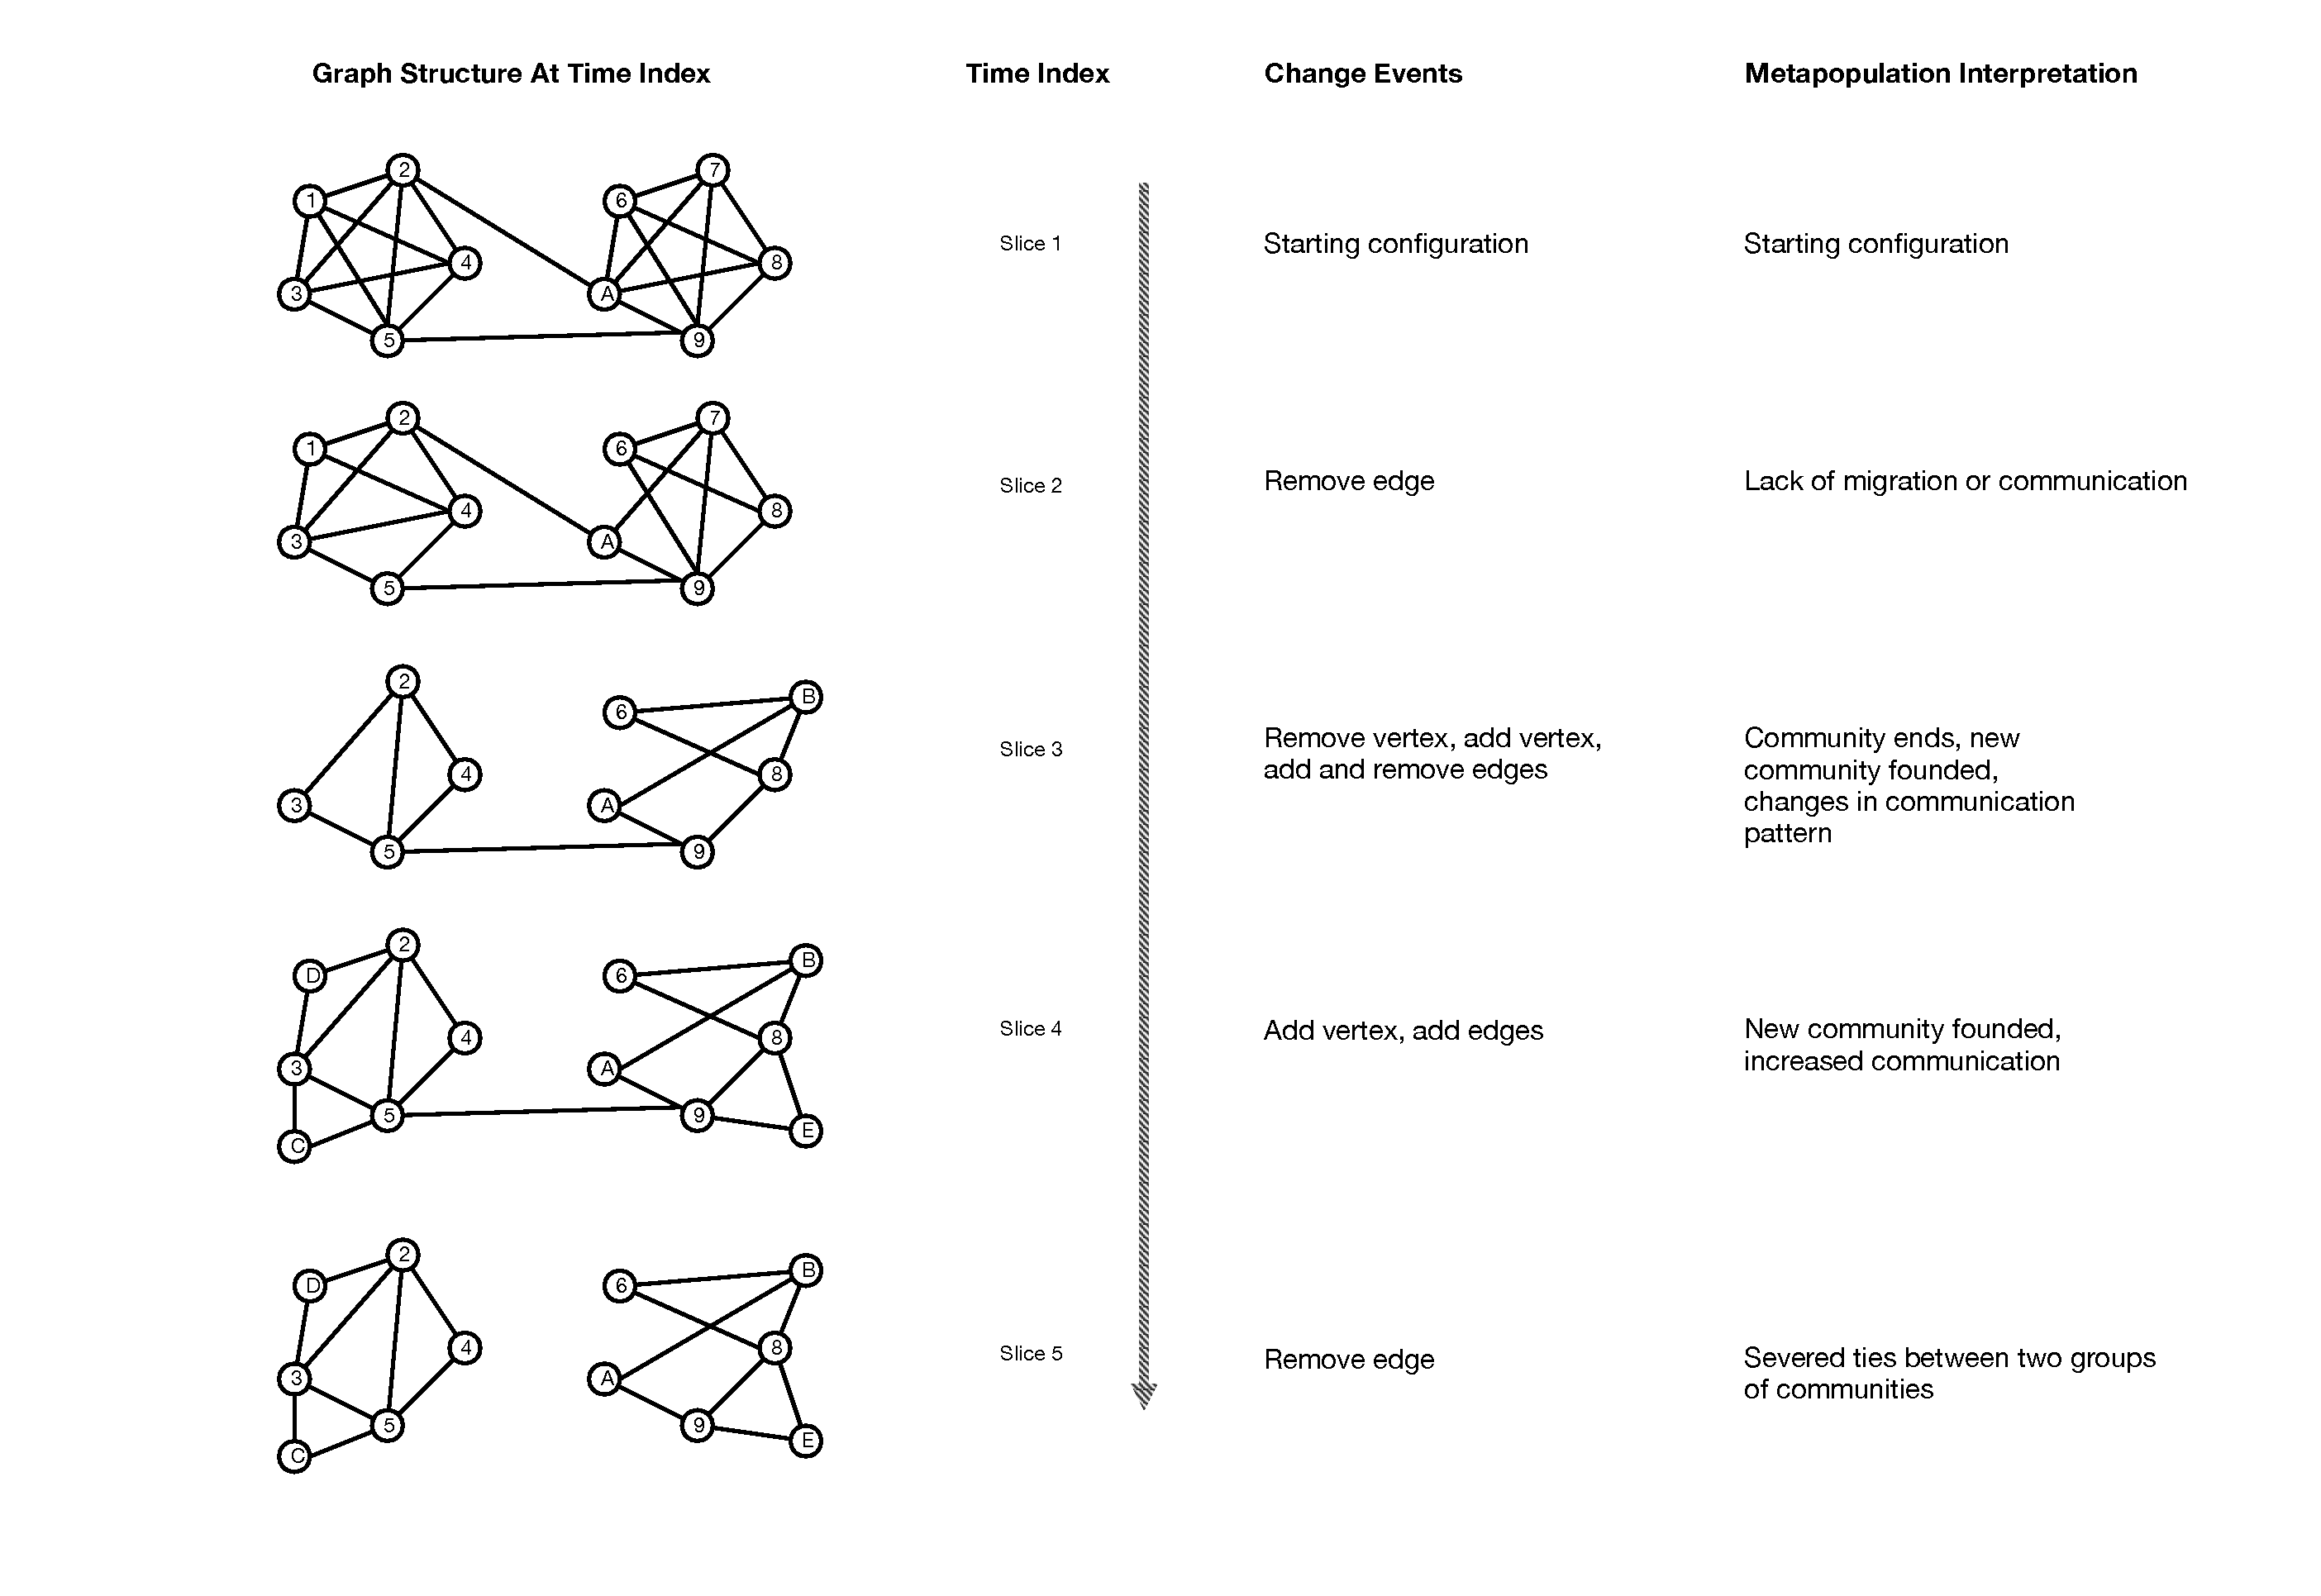
\includegraphics[scale=0.25]{graphics/multipleseriation/interval-temporal-network-with-interpretation.pdf}
    \caption{Example of an interval temporal network, which can be interpreted as a regional transmission scenario of the lineage-splitting type, with vertices representing communities, edges representing interaction and migration, and changes between subgraphs in the sequence representing changes in patterns of transmission, and the establishment and loss of communities, over time.}
    \label{metapop:fig:itn-example}
    \end{figure}
    
    
    In the present study, each of the four scenarios given is represented by a number of randomly generated interval temporal networks, that follow the overall structural pattern of the scenario.  Each scenario is constructed as a series of ``slices'' as depicted in Figure \ref{metapop:fig:itn-example}, with randomly chosen edge ``wirings'' that follow the needed pattern:  complete or nearest neighbor plus infrequent long-distance links.  In the case of lineage coalescent or splitting scenarios, the vertices that belong to the non-communicating components are randomly assigned and then links broken either starting with or ending at a designated time step.  This process of building replicas of interval temporal networks allows us to randomize over the details of network structure, to ensure that results are not idiosyncratic.\footnote{All of the experiments described in this study were created with the software located at \url{https://github.com/mmadsen/seriationct}.  The subdirectory \textbf{graphs} contains a number of standalone progams written in Python 2.7.  Each is a ``generator'' for transmission scenarios as interval temporal networks, represented as a number of slices stored in GML (Graph Modeling Language) format.}
    
    \begin{figure}[p!]
    \centering
    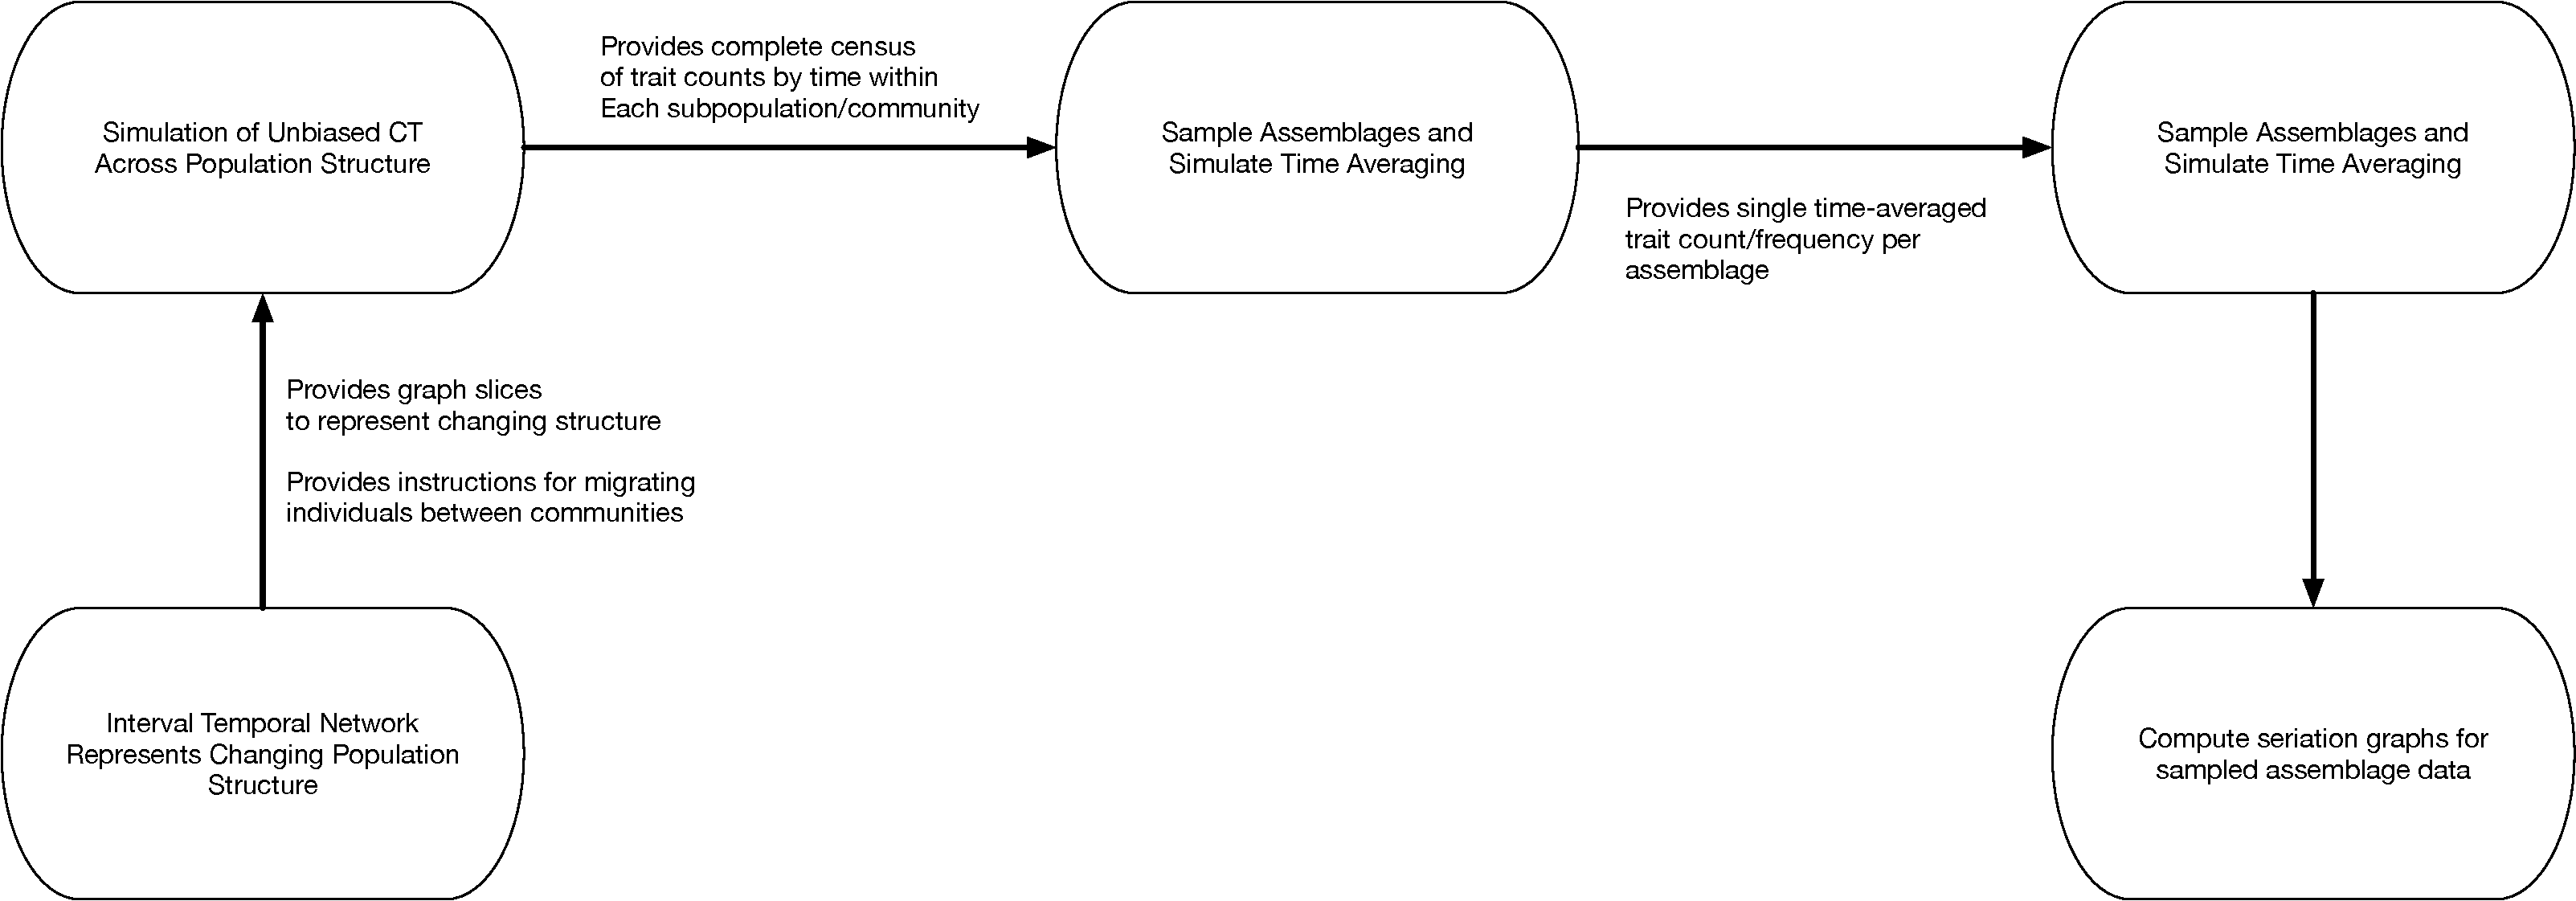
\includegraphics[scale=0.35,angle=90]{graphics/multipleseriation/simulation-sampling-seriation-flowchart.pdf}
    \caption{Flowchart for simulated data generation from each transmission scenario.  Samples of transmitted traits from each community in the transmission scenario are then aggregated in realistic ways and then the resulting trait frequencies are seriated using the IDSS seriation algorithm \citep{Lipo2015}, to produce seriation graphs as output.}
    \label{metapop:fig:simulation-flowchart}
    \end{figure}
    
    \section{Methods}\label{metapop:sec:methods}
    
    \subsection{Study Design}\label{metapop:sec:study-design}
    
    The goal in this study is to determine whether it is possible, given only the seriation graphs derived from simulations of cultural transmission in the four regional transmission histories described in the previous section, to quantitatively identify the proper data generating model. Specifially, our goal is to determine whether the structure and topology of the resulting seriation graphs is diagnostic of the transmission scenario used to generate the data.  This test is thus one that seeks to determine \emph{equifinality between transmission scenarios}, and whether our observable tools---seriation graphs---have discriminatory power.  The data generating half of the study proceeds as shown in Figure \ref{metapop:fig:simulation-flowchart}.    
    
    % Once the data generation is complete, the result is a collection of seriation graphs, each labeled with the transmission scenario under which it was generated.  An illustrative example of a simulated seriation graph is shown in Figure \ref{metapop:fig:seriation-graph-merge}, drawn from one of the ``lineage coalescence'' transmission scenarios.\footnote{Raw data and intermediate data files for the present study are located in two Github repositories.  The first records experiments in developing the transmission scenarios and understanding the level of detail that might be promising to study in an initial exploration: \url{https://github.com/mmadsen/experiment-seriation-classification}.  The second repository records experiments specifically reported here as results, using the statistical measures of seriation structure and classifier model reported:  \url{https://github.com/mmadsen/experiment-networkmkodel-identification-diss}.}
    
    % \begin{figure}[ht]
    % \centering
    % \includegraphics[scale=0.25]{graphics/multipleseriation/seriationct-27-merge-example.png}
    % \caption{Example of a seriation graph taken from a ``lineage coalescence'' transmission scenario.  Numbers in each vertex identify the simulated assemblage, and the raw simulation graph has been annotated with the line weight, with light borders indicating assemblages whose temporal position was early in the simulation, with progressively heavy line weights over time.  Shape identifies spatial clusters of communities.  In general this solution depicts two lineages merging to form one large intercommunicating regional population: two clusters represented by diamonds, and earlier circles begin sharing traits with two communities in the cluster represented by squares, and subsequent sharing renders the entire regional population intercommunicating with the same history of cultural traits over time.}
    % \label{metapop:fig:seriation-graph-merge}
    % \end{figure}
    
    \begin{figure}[p!]
    \centering
    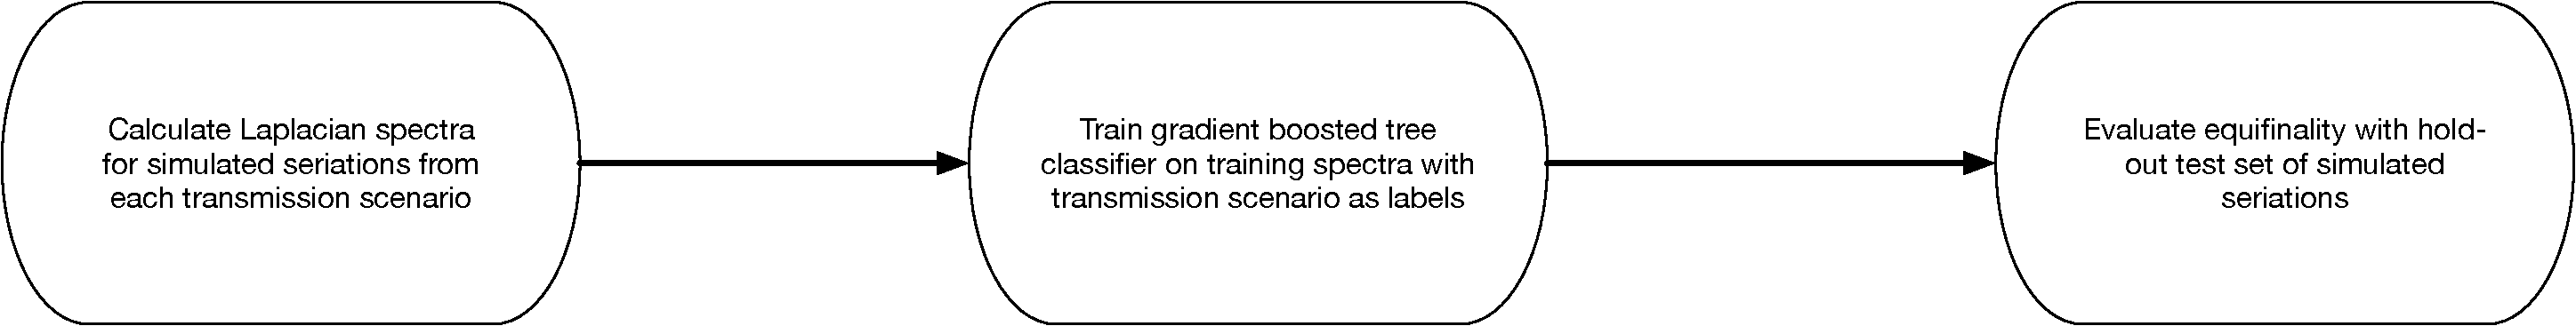
\includegraphics[scale=0.35,angle=90]{graphics/multipleseriation/theoretical-classification-equifinality-workflow.pdf}
    \caption{Flowchart for evaluating equifinality among the four candidate transmission scenarios.  Simulated seriation graphs from each model are rendered numerically using their Laplacian eigenvalue spectrum, and these eigenvalues are employed as predictor variables to train a gradient boosted tree classifier, which is then tested for predictive accuracy (and the lack of equifinality) on a hold-out set of seriation graphs.}
    \label{metapop:fig:equifinality-assessement-flowchart}
    \end{figure}
    
    Given a large sample of simulated seriations, equifinality among theoretical transmission scenarios is evaluated using a machine learning classifer (the same approach taken in Chapter \ref{chap:ctmixtures-paper}).  In order to train a classifier model, we first transform the seriation graphs into a numerical representation using their Laplacian spectrum (see Section \ref{metapop:sec:structure-seriations}.  The data are randomly split into a training set, and a hold-out test set to evaluate equifinality in terms of classifier accuracy.  Accuracy will be evaluated using the confusion matrix of correct and erroneous predictions, to determine which pairs of transmission histories are distinguishable, and which if any, display equifinality at the theoretical level.  Figure \ref{metapop:fig:equifinality-assessement-flowchart} depicts this workflow.
    
    
    \subsection{Quantifying The Structure of Seriation Solution Graphs}\label{metapop:sec:structure-seriations}
    
    In order to make comparisons between seriation graphs, and determine our ability to predict which transmission scenario generated a particular graph, we need to quantify something about the structure and topology of the graphs.  There are many types of graph metrics, but many are applicable to general graphs which contain circuits and loops \citep{chebotarev2013studying,diestel2010graph}.  The seriation graphs being constructed here are trees and have a single connected component by construction, rendering many classical graph metrics useless.  Instead, we turn to algebraic and spectral graph theory, which characterize the properties of trees and general graphs using the numerical properties or ``spectra'' of the various matrices associated with a graph \citep{banerjee2008spectrum,beineke2004topics,chung1997spectral,godsil2001algebraic}.
    
    \begin{figure}[ht]
    \centering
    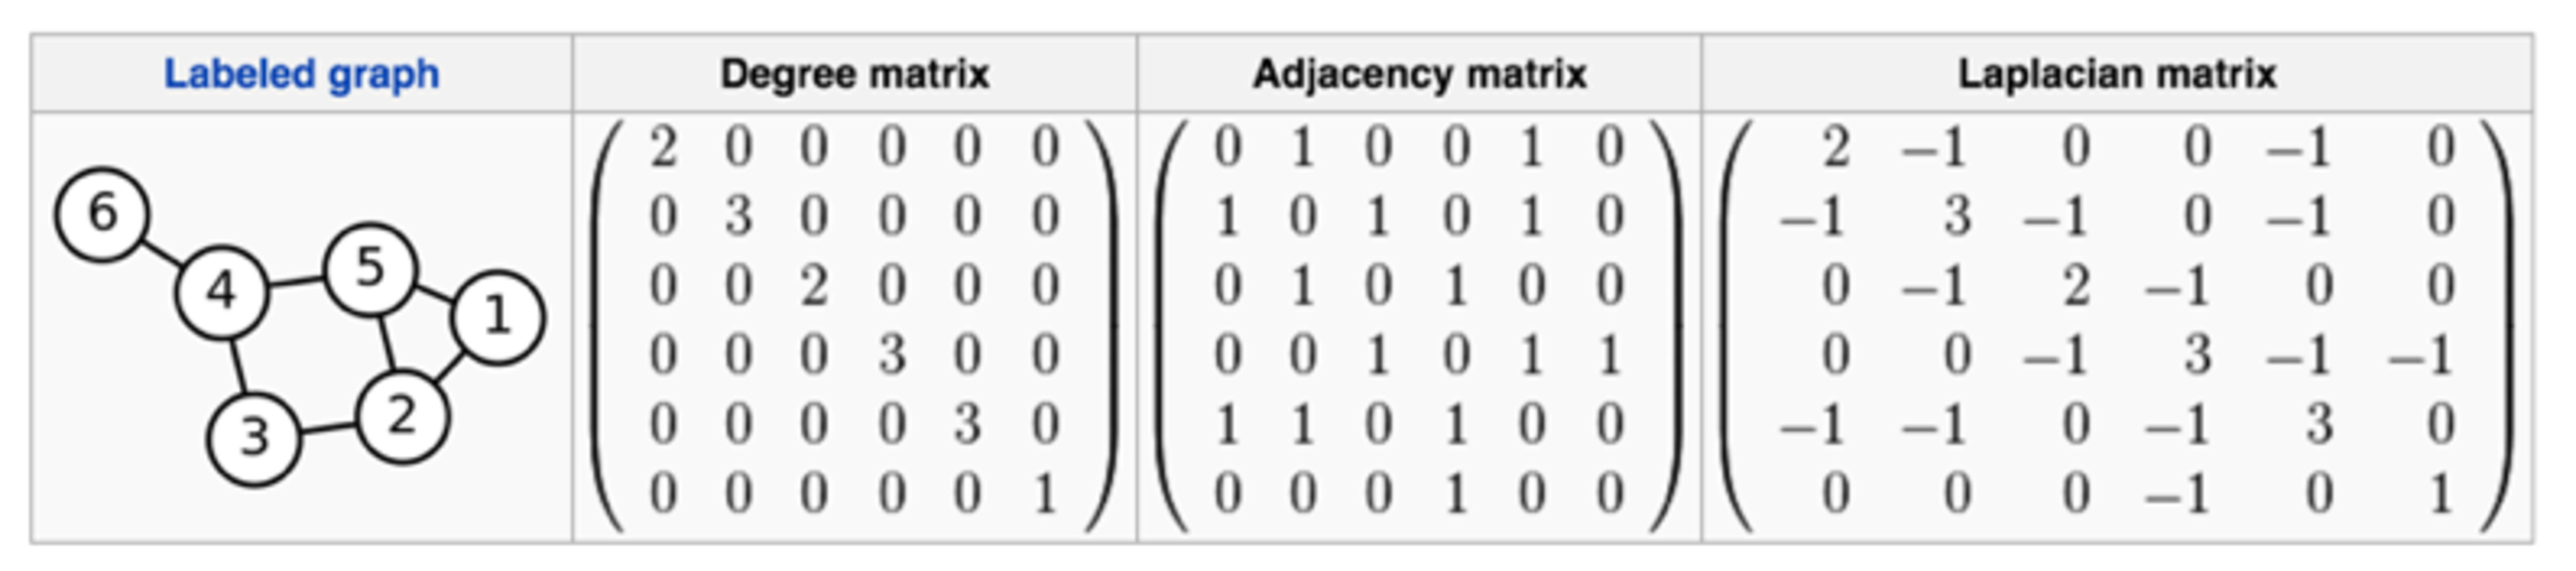
\includegraphics[scale=0.35]{graphics/multipleseriation/laplacian-matrix-for-graph.pdf}
    \caption{Simple example of calculating the Laplacian matrix for a small general graph example.  The basic Laplacian matrix is simply the element-wise difference between the degree and adjacency matrices.}
    \label{metapop:fig:laplacian-example}
    \end{figure}
    
    The ``structure'' of seriation graphs is captured in two general characteristics:  the number of branches and neighbors that assemblages possess, and the distances between assemblages.  The more a seriation is long and linear, the longer the average ``distance'' along the tree two assemblages chosen at random will be, and the more ``branched'' and reticulate the seriation is, the more average distances will decline, even as average vertex degree increases.  These intuitions are captured neatly in the \emph{Laplacian} matrix of a graph, which is defined as the difference between the ``degree matrix'' and the ``adjacency matrix'', as demonstrated for a simple example in Figure \ref{metapop:fig:laplacian-example}.  The degree matrix is a diagonal matrix where the entries along the diagonal record the number of edges attached to each vertex (i.e., vertex degree).  The adjacency matrix (for an unweighted, undirected graph, with no self-loops) has zeroes on the  diagonal, while the off-diagonal elements contain 1 if an edge is present between two vertices, and zero otherwise.  The Laplacian matrix thus encodes information about a graph's connectivity.  The ``spectrum'' is then simply the eigenvalues (and their multiplicities) of the Laplacian matrix.  
    
    Certain classes of graphs have spectra that contains every bit of information possible about the graph, and are thus ``determined'' by their spectra (e.g., finite star-like trees and the complete graphs).  In most other cases, spectra define equivalence classes of graphs with very similar structure.  Two graphs with the same spectrum of eigenvalues (and multiplicities) are \emph{cospectral} and share the same connectivity pattern even if they are not identical or isomorphic.  Further, even if two graphs are not isomorphic or cospectral, their eigenvalue spectra will be more similar to the degree they share common connectivity structures.  These properties make the Laplacian spectrum a compact numerical way to capture the structure of a graph and compare it to many other graphs.  Thus, in examining the degree to which we can predict the transmission scenario which generated a given seriation graph, what we are really asking is whether we can construct a clean partition or clustering of graph spectra arising from the four transmission scenarios given in Section \ref{metapop:sec:transmission-scenarios}.  In this study, I employed the Python \emph{NetworkX} library to calculate Laplacian matrices and spectra for seriation graphs.
    
    \subsection{Simulation of Cultural Transmission on Interval Temporal Networks}\label{metapop:sec:simulation}
    
    Simulation of cultural transmission within the interval temporal networks which represent the transmission scenarios listed in Section \ref{metapop:sec:transmission-scenarios} employ the standard unbiased copying model, since previous work demonstrates that it is difficult or impossible to detect more detailed transmission biases from the kind of coarse-grained data this study targets (see Chapter \ref{chap:timeaveraging-paper} for more details on the standard Wright-Fisher representation of unbiased cultural transmission).  The simulations were performed with a custom Python library, \emph{SeriationCT} written by the author, which adapts the \emph{SimuPOP} forward-time pouplation genetics simulation package to employ interval temporal networks as population structures, and performs the necessary sampling and temporal aggregation to simulate time averaged archaeological assemblages.\footnote{SeriationCT is open source software, available on Github at \url{https://github.com/mmadsen/seriationct}.  SimuPOP was written by Bo Peng, and is available on Github at \url{https://github.com/BoPeng/simuPOP}, and documented in his book \citep{peng2012forward}.}
    
    \begin{table}[h]
    \begin{tabular}{lc}
    \hline
    Parameter & Value or Interval \\
    \hline
    Innovation rate (in $\theta$ scaled units)  & $[0.00005, 0.0001]$   \\
    Simulation length & 10000 steps \\
    Sample fraction & 0.5 \\
    Migration fraction (between communities) & [0.05, 0.1] \\
    Individual population size & 250 \\
    Number of trait dimensions (loci) & 3 \\
    Initial traits per dimension & 5 \\
    \hline
    \end{tabular}
    
    \caption{Parameters for simulation runs across the four models studied.  Intervals are treated as prior distributions, and each simulation run is assigned values derived from a uniform random sample on the interval indicated.  Single values are applied to every simulation run, and represent a point prior.)}
    \label{metapop:tab:simulation-parameters}
    \end{table}
    
    Specifically, simulations operate in the following manner:
    
    \begin{itemize}
        \item Each individual is characterized by 3 dimensions of variation, which start out having 5 initial traits in the population;
        \item Innovation follows the standard ``infinite alleles'' model of mutation/innovation;
        \item At each time step, individuals have a probability of copying a trait from a randomly chosen individual or keeping their existing trait set.  Copying occurs within the local population only;
        \item At each time step, there is a probability of individuals moving between communities.  Movement is governed by a migration rate probability and strictly follows the edge pattern of the interval temporal network model in force for that simulation run, at that time step;
        \item At specific time steps, the interval temporal network defines changes to the connections between communities, and that some communities may go away, or new communities coming to be;
        \item New communities, should they arise, are seeded with individuals from the neighboring communities that possess edges in the network to the new community, to create a consistent sample of cultural continuity given the transmission scenario being simulated;
        \item At each time step, the frequencies of traits at each locus or dimension are tabulated, as are the cross-tabulation of ``classes'' formed by intersecting the loci;
        \item Class frequencies are aggregated over the entire duration that a community (vertex) exists in the interval temporal network model, to form time averaged ``assemblages'' for seriation analysis;
        \item Before performing seriations, assemblages were sampled from all of those available in a given simulation run, over the entire time course.  This simulates our partial view of any given regional archaeological record given what we have collected or excavated compared to the totality of the record.
    \end{itemize}
    
    Simulations were run with the parameters given in Table \ref{metapop:tab:simulation-parameters}, with parameter ranges treated as ``prior distributions'' and sampled uniformly.  This allows the simulation results to be treated as a proper Monte Carlo sampling of the space formed by the priors, for approximate Bayesian computation and other analytic methods.  500 simulations were performed for each scenario.
    
    Seriations were performed using the Python \emph{IDSS} seriation package, written by Carl Lipo and the author for our 2015 paper on iterative deterministic seriation solutions, which introduced seriation graphs \citep{Lipo2015}.\footnote{The IDSS package is open-source software, freely available at \url{https://github.com/clipo/idss-seriation}.}  Raw simulation results, all parameter choices and shell scripts to run each stage of the ITN creation, simulation, resampling, and seriation pipeline, are available in a Github repository (\url{https://github.com/mmadsen/experiment-seriation-classification}).\footnote{Additional experiments and prototypes for performing this kind of classification of transmission scenarios are located in the repository \url{https://github.com/mmadsen/experiment-networkmkodel-identification-diss}, and discussed online at \url{http://notebook.madsenlab.org}.}  Not every random sampling of assemblages from a simulation run yielded data which could be seriated due to the vagaries of sampling.  The final number of valid solutions across the four scenarios was 1946.
    
    \subsection{Classifier Training and Accuracy Evaluation}\label{metapop:sec:classifier}
    
    This study employed the same gradient boosted tree classifier model employed in my previous work on equfinality and cultural transmission (see Chapter \ref{chap:ctmixtures-paper}).  The simulated seriation graphs were randomly split into a 90\% training set and a 10\% hold-out test set, within each transmission scenario.  Each seriation graph was transformed into its Laplacian eigenvalue spectrum using a utility library of \emph{scikit-learn} compatible statistical functions maintained on Github at \url{https://github.com/mmadsen/sklearn-mmadsen}.  The resulting eigenvalue spectra became the input predictor variables for the gradient boosted classifier with numerical labels denoting each of the four transmission scenarios.  
    For this study I employed the gradient boosting implementation in the Python \emph{scikit-learn} package.  Optimal hyperparameters were found by optimization grid search with 3-fold cross validation, with learning rates ranging from 5.0 down to 0.01, and the number of trees from 10 to 500.  Optimal performance on the training set was achieved with learning rate 0.05 and 500 trees.  Final results were obtained by predicting the transmission scenario for each seriation graph in the hold-out test set in the same manner, and calculating the overall accuracy, F1 score, precision, and recall for the resulting confusion matrix.   The test set comprised 194 seriation graphs spread across the four transmission scenarios.
    
    \section{Results}\label{metapop:sec:results}
    
    
    
    \subsection{Equifinality Analysis of Transmission Scenarios with Simulated Data}\label{metapop:sec:results-simulation}
    
    \begin{figure}[ht]
    \centering
    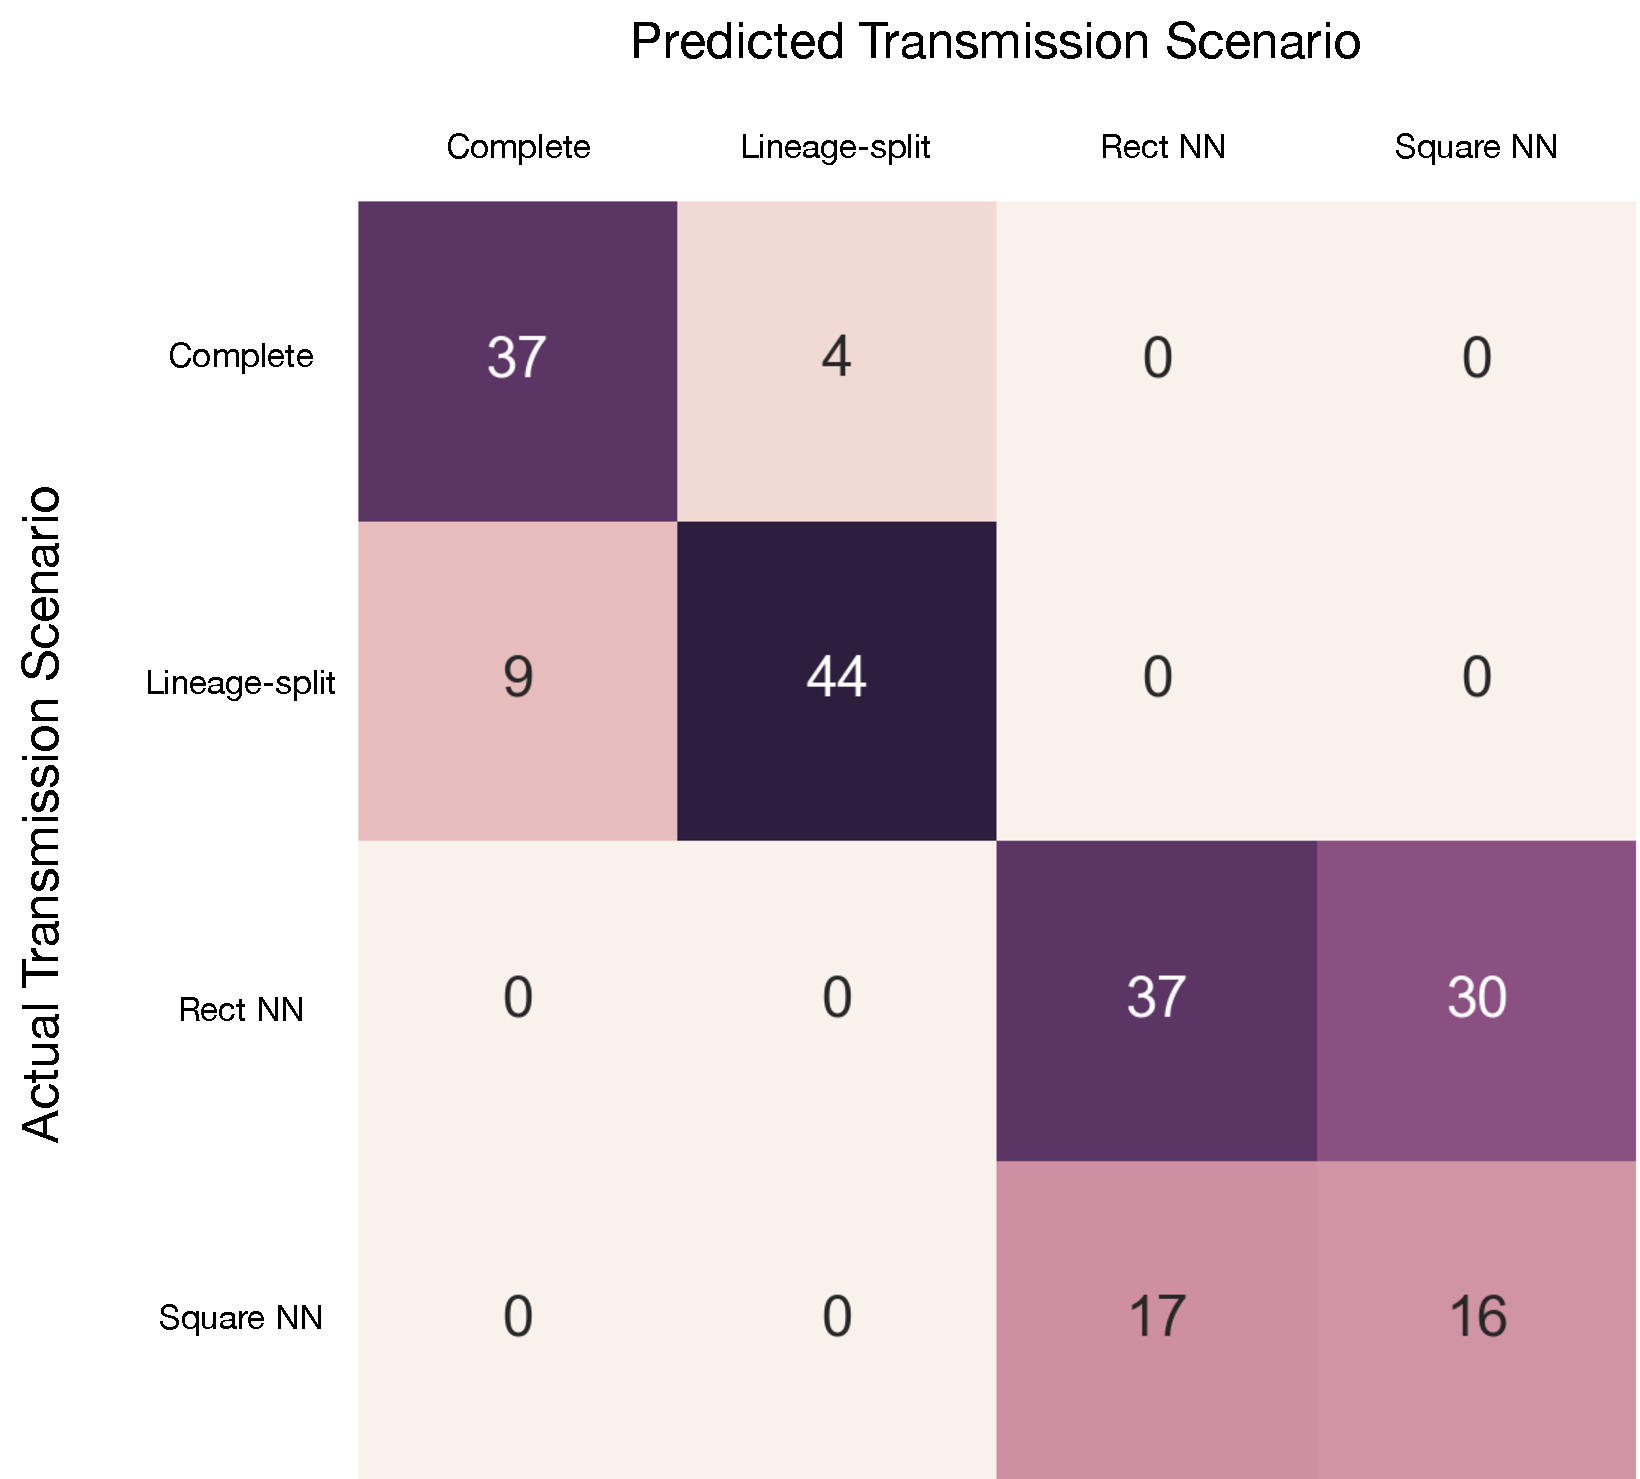
\includegraphics[scale=0.40]{graphics/multipleseriation/metapop-confusion-matrix.pdf}
    \caption{Classifier results for four regional cultural transmission history scenarios, using Laplacian spectra to determine whether seriation graphs from simulations of cultural transmission under each scenario are cleanly separable.  Results refer to evaluation of the 10\% hold-out test set of 194 seriation graphs.}
    \label{metapop:fig:confusion-matrix-testset}
    \end{figure}
    
    The results of equifinality analysis between the four transmission scenarios are given in Figure \ref{metapop:fig:confusion-matrix-testset}.  The confusion matrix has correct assignments on the diagonal:  the predicted transmission scenario matches the actual transmission scenario under which a particular simulation result was generated.  In general, accuracy is only 69.1\%, but this is driven down mainly by the inability to distinguish between our two variants of nearest-neighbor transmission scenarios.  The F1 scores for cases actually coming from complete networks was 0.85 and 0.87 for lineage-split scenarios.  It is also quite clear that one can distinguish between complete networks, lineage-splits, and nearest-neighbor scenarios \emph{in general}, given no errors. But it seems less clear that the spatial ``shape'' of the contact network has much effect on the eventual Laplacian spectrum of the seriation graphs, although this should be a major focus of followup work given the small numbers of different transmission scenarios tested.  
    
    In general, these results are encouraging for the approach studied here.  Seriation graphs may, with appropriate choice of scenarios to contrast, be capable of being statistically identified as to the equivalence class of regional cultural transmission scenarios that drove the empirical cases we see in prehistory. 
    
    \subsection{Analysis of Lower Mississippi River Valley Ceramic Data}\label{metapop:sec:results-lmv}
    
    \begin{figure}[ht]
    \centering
    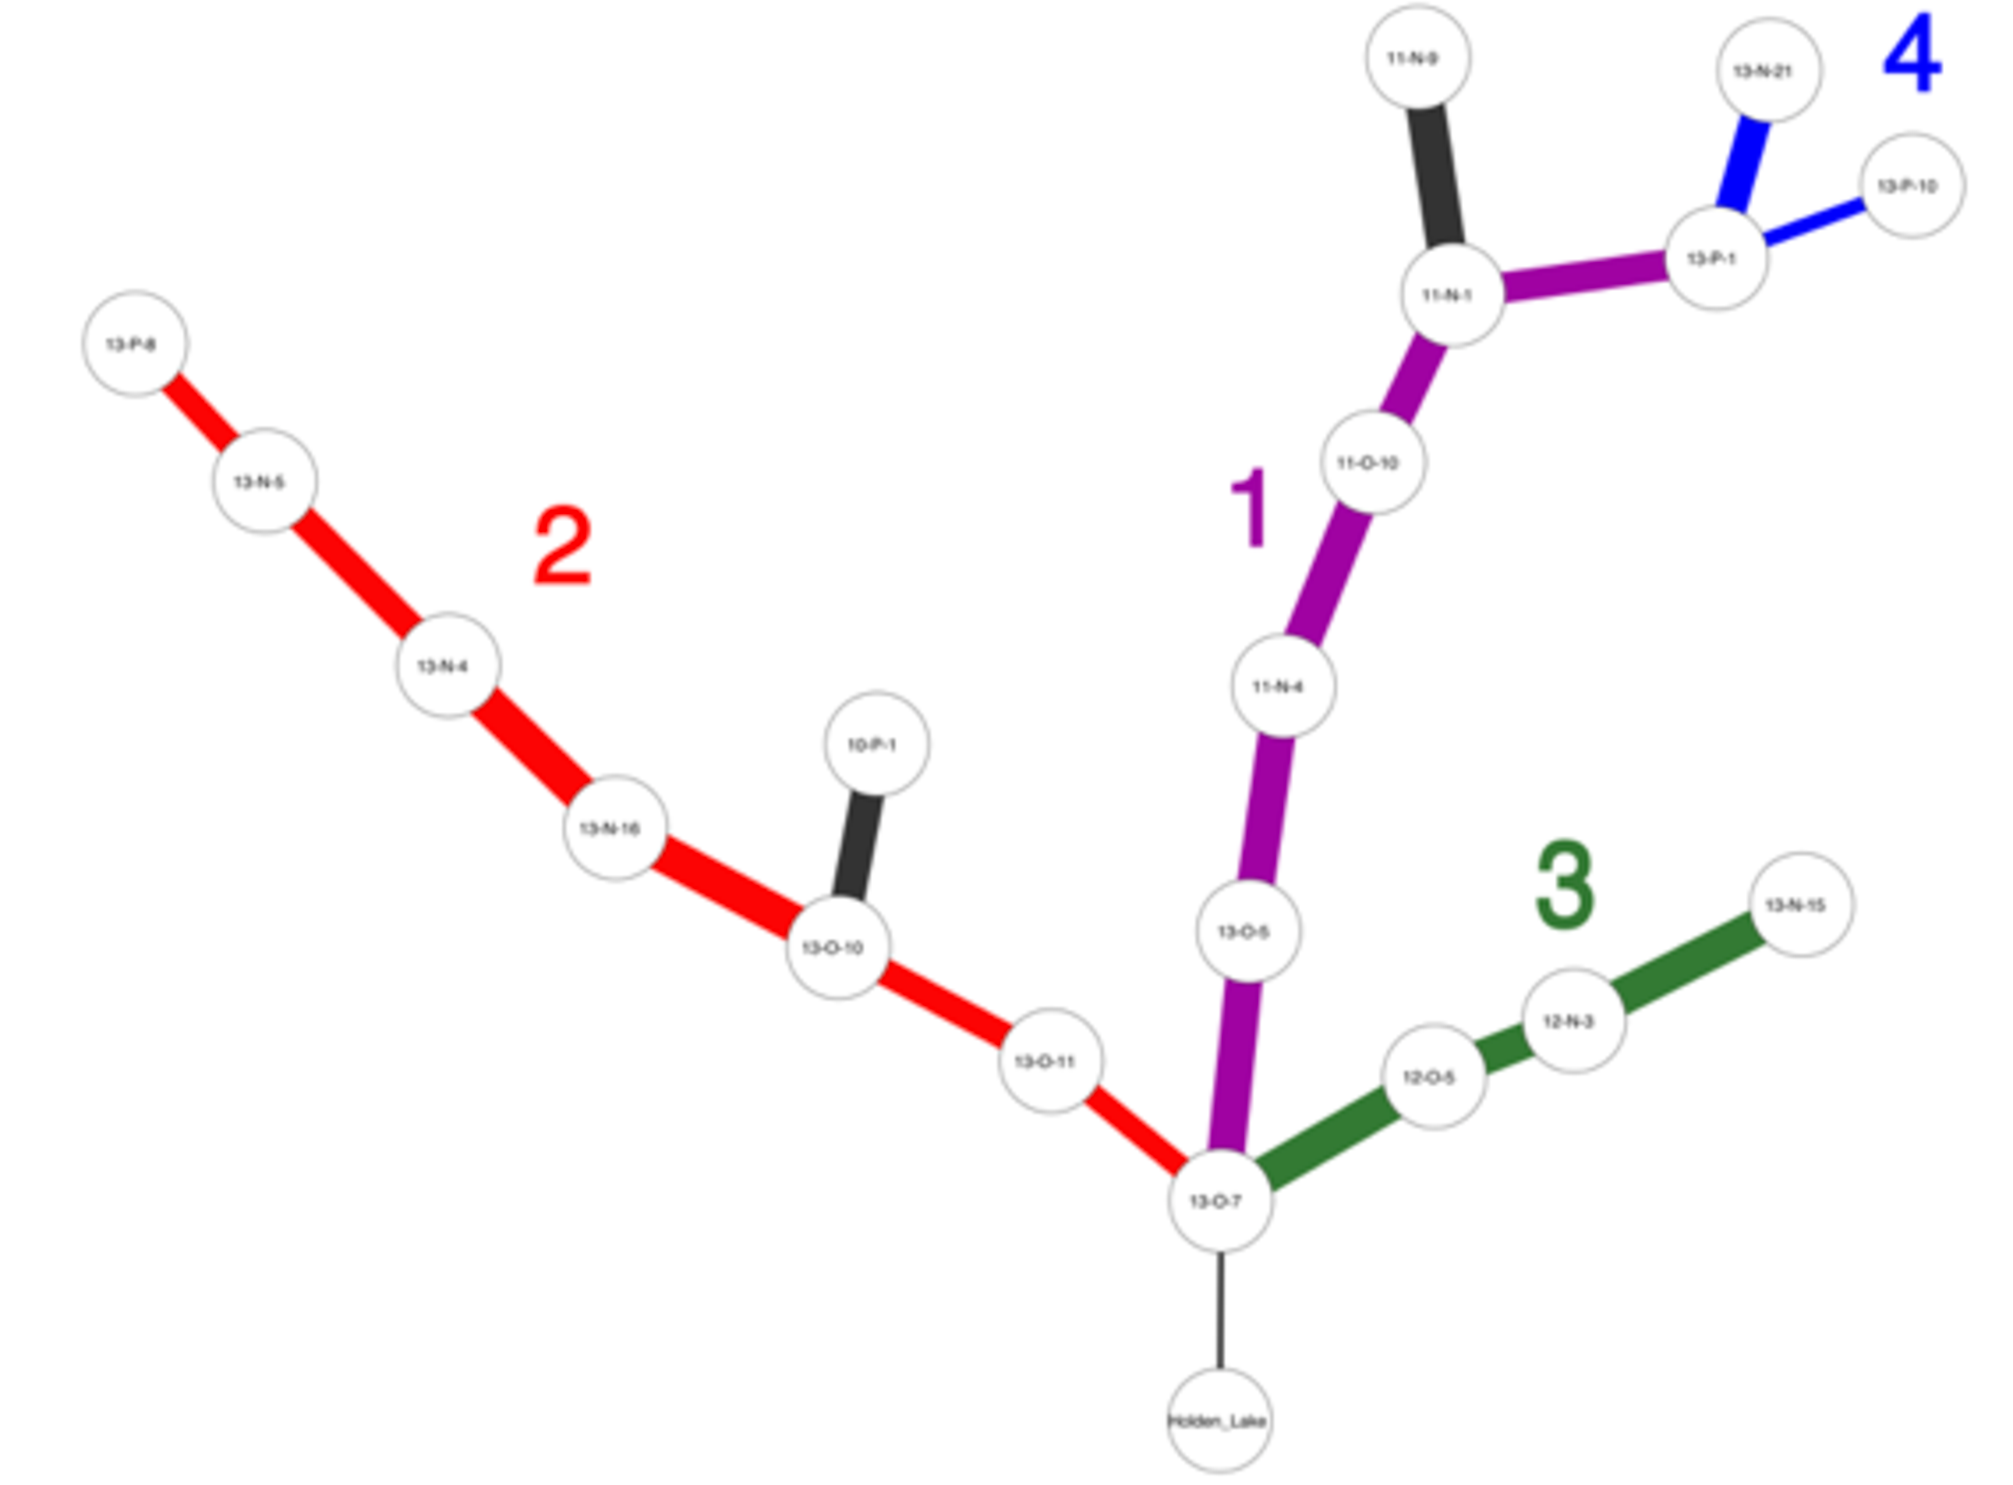
\includegraphics[scale=0.5]{graphics/multipleseriation/pfg-seriation-graph-minmax.pdf}
    \caption{Seriation graph for PFG \citeyearpar{Phillips1951} ceramic assemblages in 
    the Lower Mississippi River Valley, as analyzed by Lipo \citeyearpar{Lipo2001a} and re-analyzed by \citet{lipomadsendunnell2015}. Colors and numbers correspond to spatial clusters as mapped in Figure \ref{metapop:fig:pfg-spatial-groupings}.}
    \label{metapop:fig:pfg-seriation-graphs}
    \end{figure}
    
    Given the trained classifier model, we can analyze empirical examples and determine the degree to which the model presents a confident prediction for the transmission scenario that might correspond to our data from prehistory.  I calculated the Laplacian spectrum for a frequency seriation result from 20 ceramic assemblages from Phillips, Ford, and Griffin's \citeyearpar{PFG1951} study of the Lower Mississsippi River Valley, as augmented and reanalyzed by Carl Lipo \citep{Lipo2001}.  The resulting seriation graph is shown in Figure \ref{metapop:fig:pfg-seriation-graphs}.  There is a clear branching structure, which Lipo interpreted in his dissertation work as reflecting an early assemblage---Holden Lake---being ancestral to other early Mississippian sites in the region, but giving rise to several somewhat independent regional ceramic traditions.  There is also clear spatial structure to this results, as shown in Figure \ref{metapop:fig:pfg-spatial-groupings}.  
    
    When we use the trained classifier with the Laplacian spectrum of this seriation graph, the predicted transmission scenario is unsurprisingly the lineage split model, with probability 0.93.  The complete graph scored 0.06 probability, with the remaining 0.01 split between both nearest neighbor models.  This example is suggestive, even though the number of possible scenarios is small.  But it demonstrates the complete method by which empirical data would be processed to identify matches with possible transmission scenarios.
    
    \begin{figure}[ht]
    \centering
    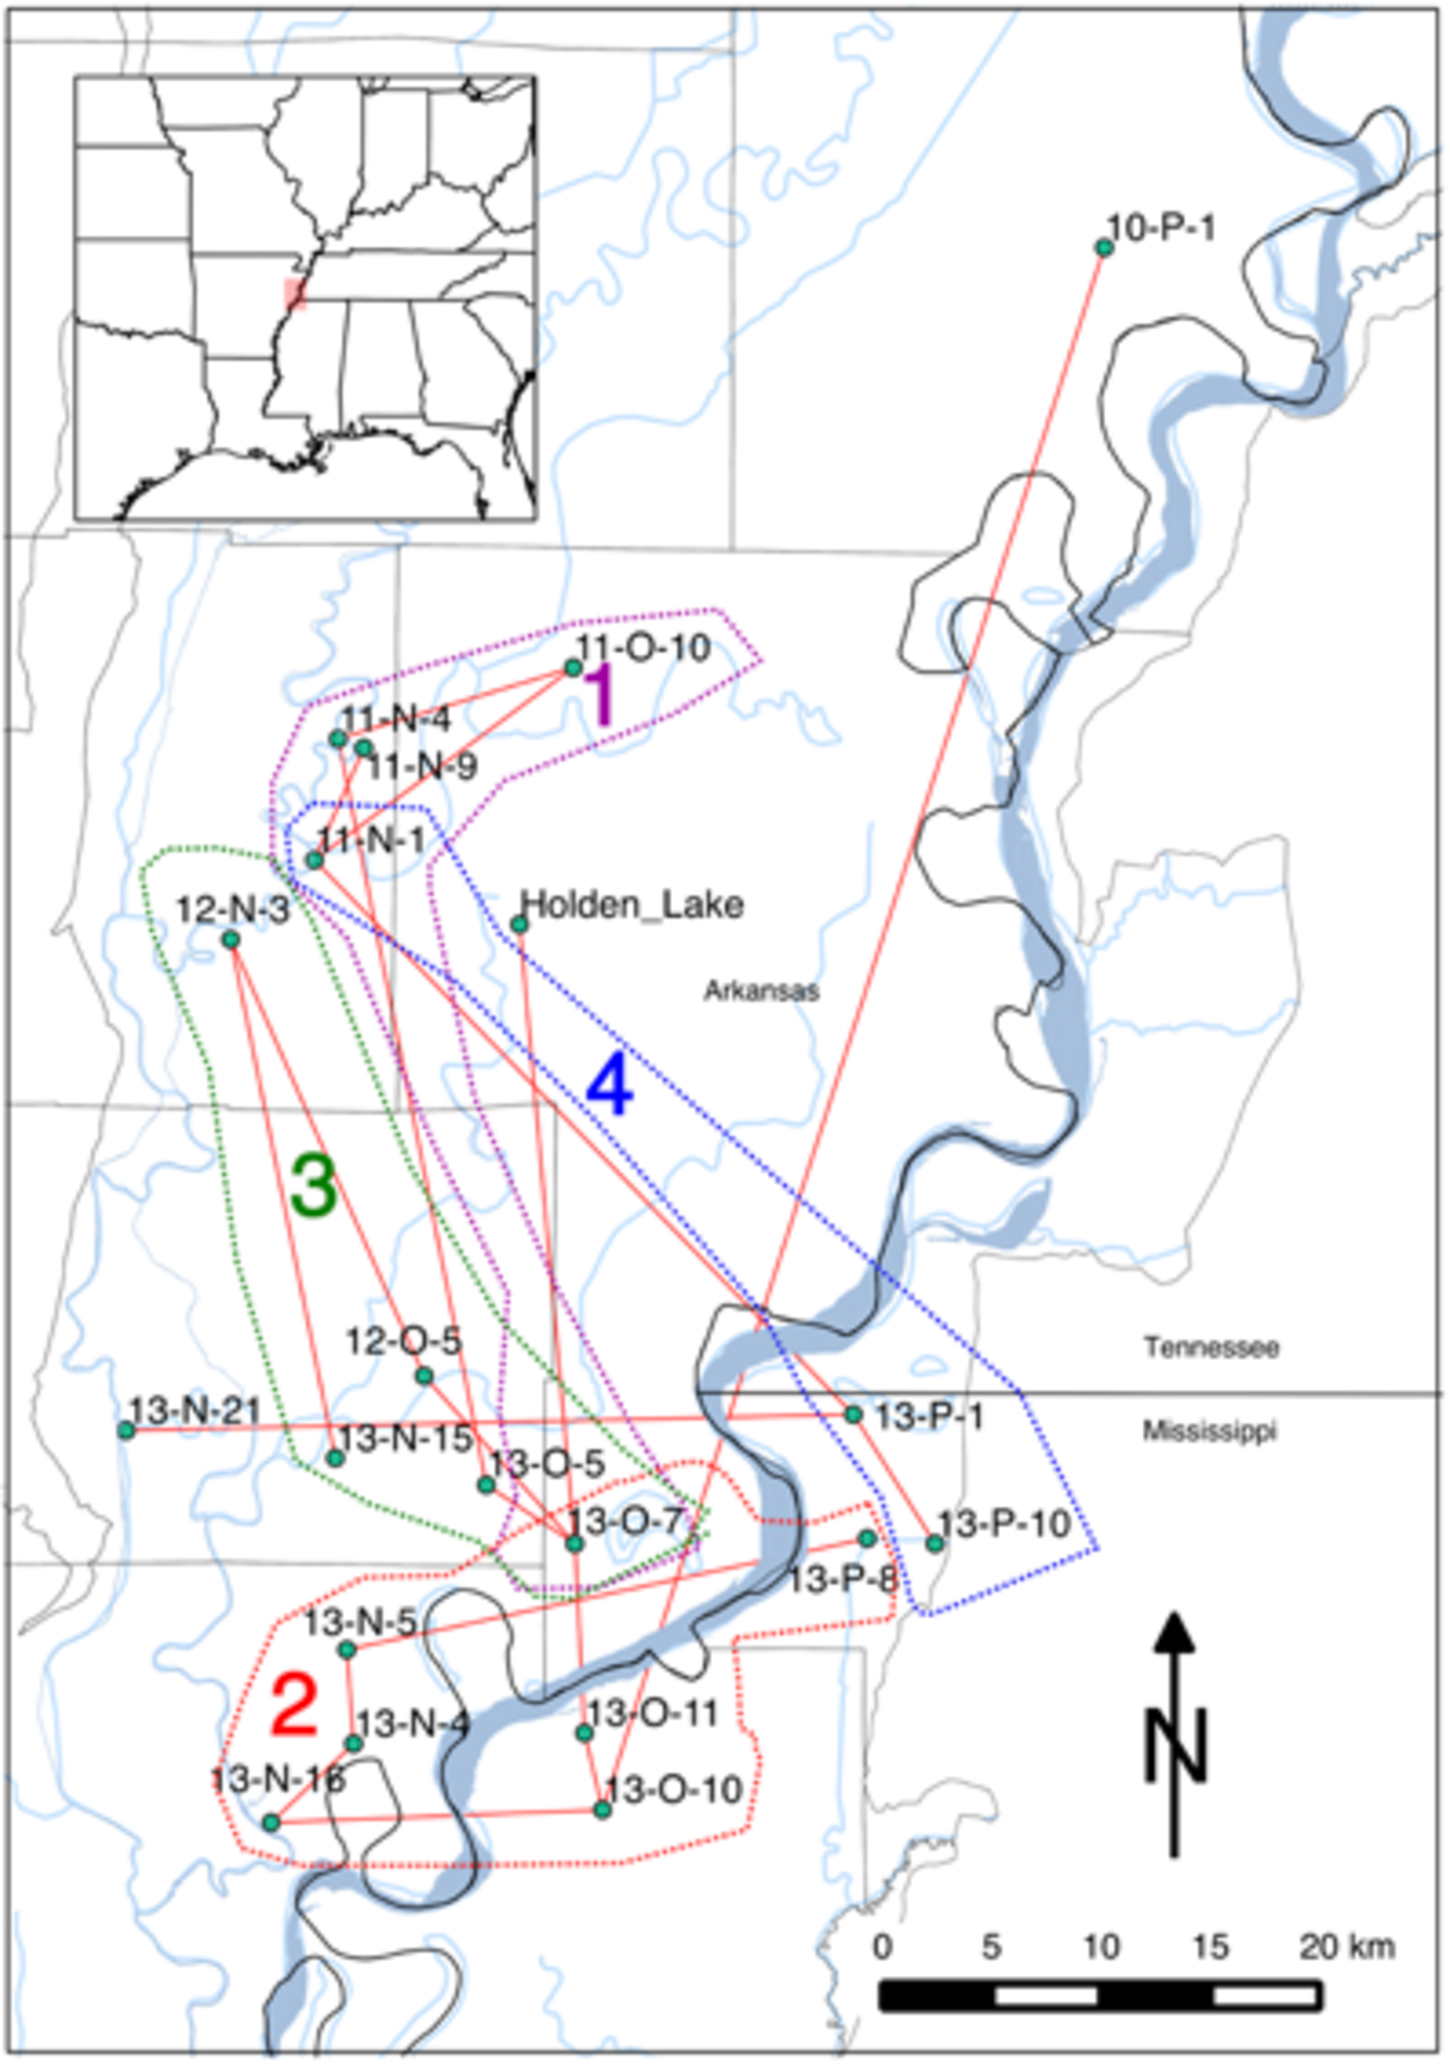
\includegraphics[scale=0.5]{graphics/multipleseriation/pfg-spatial.pdf}
    \caption{Spatial distribution of ceramic assemblages from 
    the Lower Mississippi River Valley, as analyzed by Lipo \citeyearpar{Lipo2001a}, corresponding to the seriation graph in Figure \ref{metapop:fig:pfg-seriation-graphs}.}
    \label{metapop:fig:pfg-spatial-groupings}
    \end{figure}
    
    
    \section{Discussion}\label{metapop:sec:discussion}
    
    \citet{OHara1988} usefully distinguished between the evolutionary \emph{chronicle}, which is simply the facts what happened when, from evolutionary \emph{history}, which is a narrative of how and why things happened the way they did.  At the macroevolutionary scale, phylogenetic methods produce tree structure which abstractly depict the chronicle of homologous relationships between taxa.  It is clear that the trees are data, not evolutionary history itself:  we still need to posit hypotheses about the processes and events which resulted in the observed trees.  This applies whether we are talking about genetic evolution with species as taxa, or cultural evolution with samples of cultural variation or individual artifacts as the taxa.  
    
    As we develop methods at the mesoscopic level, making use of class frequency data to attempt to study evolutionary pheneomena within regions over time scales of decades or a century, we should keep the distinction between chronicle and history firmly in mind.  In this study, I have attempted to develop a computational method for determining the statistical fit between seriation graphs (the \emph{chronicle}) and interval temporal network models which formalize the regional history of cultural transmission (the \emph{history}).  That method employs a modified seriation method which produces graphs rather than linear orderings if the data require it; the branchings in seriation graphs indicate relationships where the history of cultural traits varies through space as well as time.  I also introduced the ``interval temporal network'' as the natural way to formalize our hypotheses about the mesoscopic history of cultural transmission within and among sedentary, nucleated populations, as those populations arise, grow, and eventually go away for various reasons.  Machine learning classifiers seem able to resolve these hypotheses (in some cases) without equifinality, although there is much to be investigated within this area of research.  
    
    Given the coarseness of the transmission scenarios studied here, it is not clear yet if we can determine from seriation graphs whether ``hierarchy'' is identifiable, although this is an important next step for the study of Late Prehistoric and Late Holocene populations in many regions.  There is some evidence that spatial information may only be weakly encoded in seriation graphs, since we could not distinguish nearest neighbor hypotheses even in simulated data with different spatial configurations.  But more controlled study about the degree to which seriations encode space and with what resolution is clearly necessary; all of our knowledge of this is anecdotal given the ``same local area'' criterion long used for seriation analysis.  
    
    Despite the potential limitations of our ability to resolve differences among theoretical models, evolutionary archaeologists will benefit from further work along these lines to develop a rigorous understanding of our ability to fit theoretical models to data at a variety of spatiotemporal scales.  Phylogenetic methods have proven their worth but answer questions at particular scales and levels of detail; methods for answering more detailed questions (while still operating with coarse-grained, time averaged data) have been lacking.  Seriation, properly construed as a method for mapping homology using all of the frequency data at our disposal, provides one such tool.  
    
    

